\documentclass[egregdoesnotlikesansseriftitles,12pt]{scrartcl}

\usepackage[T1]{fontenc}
\usepackage[utf8]{inputenc}

\usepackage{adjustbox}
\usepackage[affil-it]{authblk}
\usepackage{amssymb}
\usepackage{color}
\usepackage{enumitem}
\usepackage{flafter}
\usepackage{floatrow}
\usepackage{graphicx}
\usepackage[hidelinks]{hyperref}
\usepackage{multirow}
\usepackage[all]{nowidow}
\usepackage{pdflscape}
\usepackage{setspace}

\newfloatcommand{capbtabbox}{table}[][\FBwidth]

\deffootnote{1.5em}{1em}{\makebox[1.5em][l]{\thefootnotemark}}
   \setlength{\skip\footins}{1.5em}
   \setlength{\footnotesep}{1em}

\renewcommand\Affilfont{\small}

\urlstyle{same}

\renewcommand{\autodot}{}

\title{Austin in the Lab}
\subtitle{Empirically Reconsidering the\\Constative--Performative Distinction}

\author[1*]{Stephan Kornmesser}
\author[1]{Alexander Max Bauer}

\affil[1]{ Department of Philosophy, University of Oldenburg, Germany}
\affil[*]{ Corresponding Author, E-Mail: \href{mailto:stephan.kornmesser@uni-oldenburg.de}{stephan.kornmesser@uni-oldenburg.de}}

\date{\small Forthcoming in \textit{Topics in Linguistics} 24 (2)}

\begin{document}
\maketitle

\vspace{\fill}
\begin{abstract}
   \noindent\textbf{Abstract:} \textit{Austin's groundbreaking distinction between constative and performative utterances and his investigation of how to act in saying something initiated a whole new research program in linguistics and philosophy of language. Within this program, the arguments and discussions concerning the constative--performative distinction are based on linguistic intuitions. However, generally, they are only based on the respective linguist's or philosopher's own intuitions. This fact makes the whole program seem incomplete because the linguistic intuitions of native speakers should be considered an important contribution which, so far, is mostly missing. With this article, we contribute to closing this gap by empirically investigating native speakers' linguistic intuitions with respect to the following four aims: Aim 1 is concerned with the question of whether Austin's criteria for distinguishing between performatives and constatives work. In order to achieve Aim 2, we introduce a new criterion for distinguishing between constatives and performatives, representing what we call the event character of performatives. For Aim 3, we evaluate Austin's presumably strongest argument to reject the constative--performative distinction which we call the Constative Expositive Argument. Aim 4 is concerned with the much-discussed question of whether performatives have truth values and, thus, are statements. In order to achieve the four aims, we present the findings of an online study comparing native speakers' responses to vignettes containing constative or performative utterances.}\\[2ex]
   \textbf{Keywords:} Pragmatics, Performative, Constative, John L. Austin, Native Speakers' Intuitions
\end{abstract}


%%%%%%%%%%%%%%%%
% INTRODUCTION %
%%%%%%%%%%%%%%%%
\clearpage
\section{Introduction}\label{sec:introduction}
In his seminal \textit{William James Lectures} (posthumously published as \textit{How to do Things with Words} in 1962), John L. Austin introduced the well-known distinction between constative and performative utterances. According to Austin's original idea, constative utterances (\textit{constatives}) express statements and, hence, are true or false. Performative utterances (\textit{performatives}) do not express statements, although they can grammatically look like utterances expressing statements, which is why Austin (1962: 4) also calls them \textit{masqueraders}. Performatives are not true or false; uttering them is \textit{to do} something. For example, utterance (1) below is a constative, expressing the statement that the earth turns around the sun, and utterance (2) is a performative by means of which the act of promising \textit{is done} or, in other words, performed.\\

(1) The earth turns around the sun.\par
(2) I promise to do the dishes.\\

\noindent The act of promising is performed \textit{in} saying, ``I promise to do the dishes''. According to Austin, (2) is -- like every action -- not true or false, but it can be successful (in Austin's words, \textit{happy}) or unsuccessful (\textit{unhappy}). For example, if there is no one in the room who is listening to my utterance, the action of promising is unsuccessful and, thus, the performative is unhappy. In contrast to this, uttering (1) is not to perform an act \textit{in} saying something but merely the act \textit{of} saying something which is true or false and, hence, (1) is a constative.

As it is well known, Austin replaced the distinction between constatives and performatives by his analyses of speech acts. However, Austin's groundbreaking distinction between constative and performative utterances and his investigation of how to act in saying something initiated a whole new research program in linguistics and philosophy of language that is extensively discussed independently of his speech act theory. Within this program, the arguments and discussions concerning the constative--performative distinction are based on linguistic intuitions. However, generally, they are only based on the respective linguist's or philosopher's own intuitions (in general, empirical studies on Austin seem scarce; notable exceptions are, i.\,a., Hansen and Chemla 2015 as well as Zahorec and colleagues forthcoming). This fact makes the whole program seem incomplete because linguistic rules and categorizations are based on linguistic conventions, and linguistic conventions are based on the linguistic intuitions of the whole linguistic community. Therefore, the linguistic intuitions of native speakers should be considered an important contribution which, so far, is mostly missing.

With this article, we contribute to closing this gap in part by empirically investigating native speaker intuitions about constative and performative utterances. In Section \ref{sec:aims}, we elaborate on the following four aims we strive to achieve empirically:

\textbf{Aim 1} is concerned with the question of whether Austin's criteria for distinguishing between performatives and constatives work. That is, we investigate whether native speakers' intuitions are in accordance with Austin's classification of constative and performative utterances.

In \textbf{Aim 2}, we introduce a new criterion for distinguishing between constatives and performatives representing the event character of performatives. We investigate whether native speakers classify utterances by means of this criterion in accordance with Austin's classification.

In \textbf{Aim 3}, we evaluate Austin's presumably strongest argument to reject the constative--performative distinction. We call it the \textit{Constative Expositive Argument} (CEA). We discuss the CEA on the basis of the evidence we obtained for Aim 1 and Aim 2.

In \textbf{Aim 4}, we consider the much-discussed question of whether performatives are statements. To this end, we evaluate the evidence we obtained in Aim 1 with respect to the question of whether performatives have truth values.

In order to achieve these aims, we conducted an online study. In Section \ref{sec:design}, we introduce our study design. In Section \ref{sec:results}, we present and discuss our results. Then, in Section \ref{sec:objections}, we discuss possible objections to our experimental setup before we sum up our findings in our final conclusions in Section \ref{sec:conclusion}.


%%%%%%%%
% AIMS %
%%%%%%%%
\section{Aims and Operationalizations}\label{sec:aims}
In the following, we introduce our four aims in more detail and operationalize the aims with respect to the studies we present in Section \ref{sec:results}.


%%%%%%%%%
% AIM 1 %
%%%%%%%%%
\subsection{Aim 1: Do native speaker's intuitions regarding Austin's criteria to distinguish between constatives and performatives lead to the same classification as predicted by Austin's theory of constatives and performatives?}

In order to answer the question of Aim 1, we need to evaluate Austin's criteria for distinguishing between constatives and performatives and then investigate whether native speakers intuitively come to the same classification with respect to these criteria as predicted by Austin's theory.

In his first lecture, Austin (1962: 5) introduces the two most fundamental criteria to distinguish between constatives and performatives: Constatives, but not performatives, have a truth value. Performatives, but not constatives, are actions. In order to investigate native speakers' intuitions, we derive the following two test questions from the two criteria.\\

\begin{addmargin}[11pt]{0pt}
   \textbf{Question Truth:} Can the utterances be true or false?\\
   
   \noindent\textbf{Question Act:} Is there an action performed with the utterance (in addition to the action of speaking)?\\
\end{addmargin}

\noindent According to Austin's theory, the answer to Question Truth should be ``yes'' for a constative and ``no'' for a performative, and the answer to Question Act should be ``no'' for a constative and ``yes'' for a performative. With respect to Question Truth and Question Act, Austin determines what we call the \textit{action character of performatives} and the \textit{statement character of constatives}. Actions cannot be true or false, and statements are not actions.

Besides Question Truth and Question Act, Austin developed several further tests and criteria to distinguish between both kinds of utterances. For example, Austin (1962: 55--57) suggests a grammatical criterion for the constative--performative distinction but immediately rejects it as being not distinctive (Austin 1962: 57--66). However, Austin (1962: 79--80) also proposed four further tests to decide whether a certain utterance is performative or constative that he did not give up subsequently. In the following, we will introduce two of the tests in order to evaluate them empirically in Section \ref{sec:results}. We refer to them as \textit{Question Doubt} and \textit{Question Deliberate}.\footnote{Austin (1962: 79--80) introduced a total of four tests. However, two of the tests should be ruled out because of a conflict with Austin's theory and because of a redundancy with Question Truth and Question Act. The first test we rule out is based on the idea that performatives are actions that can only be done by uttering the performative and, thus, could not be performed without uttering it. However, this test turns out to be inappropriate since it conflicts with Austin's comments on conventional actions. According to Austin (1962: 18--19), performatives are a subclass of conventional actions. Besides performatives, there are other conventional actions like rituals or ceremonials that can be performed non-linguistically. Therefore, there are conventional actions that can be performed without saying anything. Now, Austin (1962: 8) points out with respect to performatives that ``[i]n very many cases it is possible to perform an act of exactly the same kind not by uttering words, whether written or spoken, but in some other way. For example, [...] I may bet with a totalisator machine by putting a coin in a slot.'' Hence, according to Austin, there are ``very many cases'' in which one and the same action can be performed by means of a performative or in a corresponding non-linguistic conventional way. Therefore, in all of these cases, the test would lead to results contradicting Austin's classification of performatives and constatives. The other test we rule out asks whether an utterance has a truth value or whether it is the doing of an action. Hence, it corresponds to the criteria of Question Truth and Question Act and, thus, is redundant.}\\

\textbf{Question Doubt:} Does it make sense to ask ``Do they really''?\\

\noindent Question Doubt asks whether one can reasonably doubt that someone is doing what they are saying. According to Austin's intuition, if the answer is ``no'', the utterance is performative, and if the answer is ``yes'', the utterance is constative. As an example, let us apply Question Doubt to the utterances (3) and (4).\\

(3) I thank (you).\par
(4) I feel grateful.\\

\noindent According to Austin (1962: 79), (3) is a performative because the speaker performs the action of thanking in uttering (3), and (4) is a constative because the speaker truly or falsely describes what they feel. The answer to Question Doubt shall provide the right categorization of (3) and (4) into constatives or performatives. With respect to utterance (3), the answer is ``no'' because it does not make sense to ask, ``Did they really thank (someone)?'' if one utters (3). The reason for this is that uttering (3) \textit{is} the action of thanking, so the speaker is obviously thanking. On the contrary, the answer to Question Doubt with respect to utterance (4) is ``yes'', because if one utters (4), it can be doubted that they feel grateful since they are describing a mental state and that description could be false.\\

\textbf{Question Deliberate:} Does it make sense to insert the adverb ``deliberately''?\\

\noindent According to Austin's intuition, if the utterance is a performative, then it is possible to insert ``deliberately'' because the utterance is the doing of an action, and, thus, it should be possible to be done deliberately. Therefore, if the answer is ``yes'', the utterance is performative, and if the answer is ``no'', the utterance is constative. For example, one can thank deliberately, but one cannot feel grateful deliberately. Note that ``deliberately'' is not inserted into the performative utterance itself but into the report of the performative utterance, which is a constative. The report of the performative utterance is constructed by changing the tense from simple present to simple past. Hence, the performative (3) becomes the constative (5), into which ``deliberately'' is inserted (6).\\

(5) I thanked (her).\par
(6) I thanked (her) deliberately.\\

\noindent To sum up, in order to achieve Aim 1, we evaluate native speakers' response to Question Truth, Act, Doubt, and Deliberate with respect to given constatives and performatives.


%%%%%%%%%
% AIM 2 %
%%%%%%%%%
\subsection{Aim 2: Can the event character of performatives be used as a criterion for distinguishing between performatives and constatives?}
In addition to Austin's test questions, we will introduce \textit{Question Time} as a further criterion for the constative--performative distinction. Question Time is based on an intrinsic property of performatives postulated by \'{E}mile Benveniste (1974: 304--305). Benveniste points out that every performative is a single event that is not repeatable. That is, every repetition of a performative would be a new event. We call this property the \textit{event character of performatives}. How can the event character of performatives be used for the constative--performative distinction? If an action is done by means of uttering a performative, this action is an event limited in time. Therefore, it is not possible to still perform this action at a later point in time. Hence, we suggest Question Time as a test to distinguish between constatives and performatives.\footnote{This test goes back to an idea of Merle Toborg. She developed this idea in an essay in an undergraduate course on Austin's (1962) \textit{How to do Things with Words}.}\\

\textbf{Question Time:} Does it make sense to ask ``Are they still doing it''?\\

\noindent According to our hypothesis, the answer to the Question Time will be ``no'' if it refers to a performative and ``yes'' if it refers to a constative. For example, with respect to utterance (3), the answer to the question is ``no'' because the action of thanking is an event that is completed with uttering (3). On the contrary, with respect to the utterance (4), the answer is ``yes'' because they could still feel grateful or not. In other words, Question Time refers to different levels of doing something: For the performative, the action to which Question Time refers is done by uttering the performative. For the constative, the action to which Question Time refers is not done by uttering the constative, but it is the action that is described, reported, and so forth, by the constative and this action usually can last in time. That is, Question Time takes advantage of these two different ways of doing something which is reflected in the constative--performative distinction.


%%%%%%%%%
% AIM 3 %
%%%%%%%%%
\subsection{Aim 3: Does Austin's Constative Expositive Argument work?}
After introducing the constative--performative distinction in his \textit{William James Lectures}, Austin himself subsequently rejected the constative--performative distinction arguing that there are no such two disjunct categories. Austin's reason for giving up the distinction is that constatives also have the properties of performatives and vice versa. That is, performatives can depend on facts or relevant states of affairs like constatives, and constatives can be considered actions like performatives, e.\,g., the action of describing, reporting, claiming, and so on (Austin 1962: 54--55, 91, Black 1963: 223--225, Forguson 1966, Warnock 1973). Austin's strongest argument against the distinction between constatives and performatives follows from his speech act theory. According to Austin (1962: 98), every performance of a locutionary act (the act of saying something) is \textit{eo ipso} the performance of an illocutionary act (the act of doing something in saying something). That is, uttering a constative is also doing, for instance, the act of describing, reporting, claiming, and so forth. In other words, constatives are like implicit performatives. For example, utterance (1) actually might be an abbreviation of the (explicit) performative\\

(7) I claim that the earth turns around the sun,\\

\noindent because in uttering (1), I implicitly perform the action of making a claim. In consequence, every utterance is a performative (Black 1963: 225).\footnote{On the other hand, there are authors that explicitly defend the constative--performative distinction against Austin by refining Austin’s definitions of performative utterances (e.\,g., Chisholm 1969: 108--110, Sesonske 1965: 467, Katz 1977: 158--160, Benveniste 1974: 299--308).} More detailed: Every constative is an expositive (as defined below) since claims, descriptions, reports and so forth are expositives. We call this argument the Constative Expositive Argument (CEA). In Aim 3, we will evaluate our data, considering whether the CEA holds.


%%%%%%%%%
% AIM 4 %
%%%%%%%%%
\subsection{Aim 4: Are performatives statements?}
As pointed out already, according to Austin (1962: 5--6) performatives do not have truth values. However, as Hornsby (2006: 904) states, Austin's point of view is rejected by the majority of post-Austinian philosophers working on performativity (see also Tsohatzidis 2018: 97--103). For example, it is prominently challenged by Lemmon (1962), Quine (1981), Heal (1974), Bach (1975), Graham (1977), and Searle (1989). According to these authors, utterances like (2) are in accordance to Austin actions, but additionally, they have a truth value and, hence, they are statements. The special character of utterances like (2) is that their truth conditions are satisfied ``simply by uttering the sentence in the right circumstances'' (Soames 2003: 127). For instance, in uttering (2), one is performing a promise, and because of this (2) rightly describes what is done, and, hence, (2) is true. From this point of view, a (happy) performative ``makes itself true'' (Quine 1981: 90) and, thus, performatives are ``verifiable by their use'' (Lemmon 1962: 88) or simply ``self-verifying'' (Heal 1974: 116--117, see Bach (1974) for another way of arguing that performatives have truth values). However, there are also authors who support Austin's view that performatives do not have truth values (e.\,g., Tsohatzidis 2018: 103--118). We will take a look at whether performatives are considered to have a truth value according to our subjects' intuitions when analyzing responses to Question Truth in Section \ref{sec:results}.


%%%%%%%%%%
% DESIGN %
%%%%%%%%%%
\section{Study Design}\label{sec:design}
To explore the questions introduced above, we designed an online study comparing subjects' responses to constatives and performatives. For this, we had to select a number of performatives to present in the study. In order to provide a wide selection, we chose one performative of each of the following five classes of performatives Austin (1962: 152--162) introduced in his twelfth lecture: \textbf{Behabitives} ``include the notion of reaction to other people's behaviour and fortunes and of attitudes and expressions of attitudes to someone else's past conduct or imminent conduct'' (159). \textbf{Verdictives} ``consist in the delivering of a finding, official or unofficial, upon evidence or reasons as to value or fact, so far as these are indistinguishable'' (152). \textbf{Exercitives} are the givings of decisions ``in favour of or against a certain course of action, or advocacy of it'' (154). \textbf{Commissives} are commitments of ``the speaker to a certain course of action'' (156). \textbf{Expositives} ``are used in acts of exposition involving the expounding of views, the conducting of arguments, and the clarifying of usages and of references'' (160).\footnote{Of course, we are aware of the fact that Austin's classification has been prominently challenged by Searle (1975, but see also criticism of Searle's classification by Siebel 2002). However, we focus on Austin's account of performatives and, thus, refer to Austin's classifications. Although we share the objections to Austin's classification, we think that choosing performatives from the classes introduced by him will provide a widespread selection of different kinds of performatives.} For every kind of performative, we devised an exemplary utterance (see Table \ref{tab:vignettes}). To each performative, we assigned a constative that was presented in exactly the same context as the respective performative. In order to investigate possible differences in perceptions between performatives and constatives, every performative was altered as slightly as possible to form a corresponding constative utterance. For example:\\

(8) I apologize for the accident. (performative, behabitive)\par
(9) I regret the accident. (assigned constative)\\

\noindent Thus, we ended up with a total of ten vignettes, as depicted in Table \ref{tab:vignettes}. In order to prevent subjects from making direct comparisons between a performative and the assigned constative, we choose a between-subjects design. That is, each subject saw only one of those ten vignettes. Each subject was then asked the five yes-or-no questions as introduced in Section \ref{sec:aims} in random order: Question Truth, Question Act, Question Doubt, Question Deliberate, and Question Time (for the exact wording, see Appendix \ref{sec:app_questions}).

\begin{table}[ht]
\resizebox{\linewidth}{!}{%
\begin{tabular}{lll}
\hline
                            &        & Vignette                                                                                                                                                                                                                  \\
\hline\hline
\multirow{2}{*}{Behabitive} & Perf.  & \begin{tabular}[c]{@{}l@{}}Petra and Hans had a bicycle crash yesterday. Hans had taken Petra's right of way and\\ collided with her. The next day he visits her and says, ``I apologize for the accident.''\end{tabular} \\
                            & Const. & \begin{tabular}[c]{@{}l@{}}Petra and Hans had a bicycle crash yesterday. Hans had taken Petra's right of way and\\ collided with her. The next day he visits her and says, ``I regret the accident.''\end{tabular}        \\
\hline
\multirow{2}{*}{Verdictive} & Perf.  & A judge says to the defendant as she pronounces the verdict, ``I hereby acquit you.''                                                                                                                                     \\
                            & Const. & A judge says to the defendant after the verdict is pronounced, ``I believe you are innocent.''                                                                                                                            \\
\hline
\multirow{2}{*}{Exercitive} & Perf.  & The president says to the inmate, ``I hereby pardon you.''                                                                                                                                                                \\
                            & Const. & The president says to the inmate, ``I believe you should be pardoned.''                                                                                                                                                   \\
\hline
\multirow{2}{*}{Commissive} & Perf.  & Petra says to Hans, ``I promise to take you to the movies.''                                                                                                                                                              \\
                            & Const. & Petra says to Hans, ``I have the intention of taking you to the movies.''                                                                                                                                                 \\
\hline
\multirow{2}{*}{Expositive} & Perf.  & Petra says to Hans, ``I claim that Leonardo DiCaprio is the most attractive man.''                                                                                                                                        \\
                            & Const. & Petra says to Hans, ``I think Leonardo DiCaprio is the most attractive man.''                                                                                                                                             \\
\hline\\[-1.5ex]
\multicolumn{3}{p{20cm}}{\footnotesize\textit{This table shows each vignette presented to subjects. Vignettes represent five classes of performatives (Behabitives, Verdictives, Exercitives, Commissives, and Expositives). For each performative (Perf.), we construced an analgoue constative (Const.). The ten vignettes were presented between subjects.}}
\caption{Vignettes}\label{tab:vignettes}
\end{tabular}}
\end{table}

Before seeing a vignette and answering these questions, subjects were greeted with a welcome text (see Appendix \ref{sec:app_welcome}) and some instructions (see Appendix \ref{sec:app_instructions}). After answering the main questions, a questionnaire was used to gain some socio-demographic information. Here, we asked subjects for their gender, age, and educational background.

To make sure that subjects read the vignettes and instructions thoroughly, we asked a control question right after the five main questions (see Appendix \ref{sec:app_control}). Only those subjects who answered this question correctly were included in our final analysis. Those $617$ subjects received a flat fee of $2.55$ euros. Another $176$ subjects were excluded from the study after failing to answer our control question correctly. As was announced beforehand, they were not compensated.

Our study was programmed in LimeSurvey (2020). It was conducted online in August and September 2021. Subjects were recruited by the private market research institute \textit{respondi} where they were randomly drawn from a pool of registered subjects from Germany.\footnote{Hence, the results presented here provide evidence concerning the constative--performative distinction in German language.} Vignettes and questions were presented to them in German. In total, $617$ subjects participated in our study. Out of our subjects, $294$ ($47.65\%$) stated to be female, $1$ ($0.16\%$) to be non-binary, and $322$ ($52.19\%$) stated to be male. The mean of their age was $48.45$ years (ranging from $18$ to $82$).


%%%%%%%%%%%
% RESULTS %
%%%%%%%%%%%
\section{Results and Discussion}\label{sec:results}
We are interested in a possible between-subjects treatment effect between performative and constative utterances. To analyze this, we perform $\chi^2$ tests -- comparing the performative and constative utterances for Behabitives, Verdictives, Exercitives, Commissives, and Expositives separately -- to examine whether there are significant differences in answering patterns. This is done question by question. Accordingly, Table \ref{tab:tests} reports absolute (and in parentheses relative) frequencies for the answers ``no'' and ``yes'' given to each of our five questions in case of the performative and constative versions of an utterance.\footnote{Data is available from \href{https://github.com/alephmembeth/speech-constative-performative/}{https://github.com/alephmembeth/speech-constative-performative/}.} For each question of each vignette, $\chi^2$ tests and Cramér's V are reported.\footnote{For the qualitative categorization of the effect size, we refer to the conventions proposed by Cohen (1988: 223--226). Accordingly, $0.1<|V|<0.29$ is considered a small effect, $0.3<|V|<0.49$ is considered a medium effect, and $0.5<|V|)$ is considered a strong effect.}

\begin{landscape}
\begin{table}[]
\resizebox{\linewidth}{!}{%
\begin{tabular}{lllcccclcccclcccclcccclcccc}
\hline
\multirow{2}{*}{Question}     & \multirow{2}{*}{Answer} &  & \multicolumn{4}{c}{Behabitive}                                                                                                                                                  &  & \multicolumn{4}{c}{Verdictive}                                                                                                                                                        &  & \multicolumn{4}{c}{Exercitive}                                                                                                                                                        &  & \multicolumn{4}{c}{Commissive}                                                                                                                                                        &  & \multicolumn{4}{c}{Expositive}                                                                                                                                                        \\\cline{4-7}\cline{9-12}\cline{14-17}\cline{19-22}\cline{24-27}
                              &                         &  & Perf.                                                    & Const.                                                   &                               &                           &  & Perf.                                                    & Const.                                                   &                                     &                           &  & Perf.                                                    & Cons.                                                    &                                     &                           &  & Perf.                                                    & Const.                                                   &                                     &                           &  & Perf.                                                    & Const.                                                   &                                     &                           \\
                              &                         &  & $n=63$                                                   & $n=56$                                                   & $p$                           & $V$                       &  & $n=62$                                                   & $n=62$                                                   & $p$                                 & $V$                       &  & $n=62$                                                   & $n=57$                                                   & $p$                                 & $V$                       &  & $n=57$                                                   & $n=67$                                                   & $p$                                 & $V$                       &  & $n=71$                                                   & $n=60$                                                   & $p$                                 & $V$                       \\
\hline\hline
\multirow{2}{*}{Truth}        & No                      &  & \begin{tabular}[c]{@{}c@{}}$16$\\ $(13.45)$\end{tabular} & \begin{tabular}[c]{@{}c@{}}$6$\\ $(5.04)$\end{tabular}   & \multirow{2}{*}{$0.039^{*}$}  & \multirow{2}{*}{$0.189$}  &  & \begin{tabular}[c]{@{}c@{}}$36$\\ $(29.03)$\end{tabular} & \begin{tabular}[c]{@{}c@{}}$10$\\ $(8.06)$\end{tabular}  & \multirow{2}{*}{$\leq 0.001^{***}$} & \multirow{2}{*}{$0.434$}  &  & \begin{tabular}[c]{@{}c@{}}$23$\\ $(19.33)$\end{tabular} & \begin{tabular}[c]{@{}c@{}}$10$\\ $(8.40)$\end{tabular}  & \multirow{2}{*}{$0.017^{*}$}        & \multirow{2}{*}{$0.218$}  &  & \begin{tabular}[c]{@{}c@{}}$13$\\ $(10.48)$\end{tabular} & \begin{tabular}[c]{@{}c@{}}$11$\\ $(8.87)$\end{tabular}  & \multirow{2}{*}{$0.369$}            & \multirow{2}{*}{$0.081$}  &  & \begin{tabular}[c]{@{}c@{}}$14$\\ $(10.69)$\end{tabular} & \begin{tabular}[c]{@{}c@{}}$8$\\ $(6.11)$\end{tabular}   & \multirow{2}{*}{$0.330$}            & \multirow{2}{*}{$0.085$}  \\
                              & Yes                     &  & \begin{tabular}[c]{@{}c@{}}$47$\\ $(39.50)$\end{tabular} & \begin{tabular}[c]{@{}c@{}}$50$\\ $(42.02)$\end{tabular} &                               &                           &  & \begin{tabular}[c]{@{}c@{}}$26$\\ $(20.97)$\end{tabular} & \begin{tabular}[c]{@{}c@{}}$52$\\ $(41.94)$\end{tabular} &                                     &                           &  & \begin{tabular}[c]{@{}c@{}}$39$\\ $(32.77)$\end{tabular} & \begin{tabular}[c]{@{}c@{}}$47$\\ $(39.50)$\end{tabular} &                                     &                           &  & \begin{tabular}[c]{@{}c@{}}$44$\\ $(35.48)$\end{tabular} & \begin{tabular}[c]{@{}c@{}}$56$\\ $(45.16)$\end{tabular} &                                     &                           &  & \begin{tabular}[c]{@{}c@{}}$57$\\ $(43.51)$\end{tabular} & \begin{tabular}[c]{@{}c@{}}$52$\\ $(39.69)$\end{tabular} &                                     &                           \\
\hline
\multirow{2}{*}{Act}          & No                      &  & \begin{tabular}[c]{@{}c@{}}$28$\\ $(23.53)$\end{tabular} & \begin{tabular}[c]{@{}c@{}}$27$\\ $(22.69)$\end{tabular} & \multirow{2}{*}{$0.681$}      & \multirow{2}{*}{$-0.038$} &  & \begin{tabular}[c]{@{}c@{}}$25$\\ $(20.16)$\end{tabular} & \begin{tabular}[c]{@{}c@{}}$38$\\ $(30.65)$\end{tabular} & \multirow{2}{*}{$0.020^{*}$}        & \multirow{2}{*}{$-0.210$} &  & \begin{tabular}[c]{@{}c@{}}$26$\\ $(21.85)$\end{tabular} & \begin{tabular}[c]{@{}c@{}}$48$\\ $(40.34)$\end{tabular} & \multirow{2}{*}{$\leq 0.001^{***}$} & \multirow{2}{*}{$-0.436$} &  & \begin{tabular}[c]{@{}c@{}}$35$\\ $(28.23)$\end{tabular} & \begin{tabular}[c]{@{}c@{}}$52$\\ $(41.94)$\end{tabular} & \multirow{2}{*}{$0.049^{*}$}        & \multirow{2}{*}{$-0.177$} &  & \begin{tabular}[c]{@{}c@{}}$56$\\ $(42.75)$\end{tabular} & \begin{tabular}[c]{@{}c@{}}$50$\\ $(38.17)$\end{tabular} & \multirow{2}{*}{$0.517$}            & \multirow{2}{*}{$-0.057$} \\
                              & Yes                     &  & \begin{tabular}[c]{@{}c@{}}$35$\\ $(29.41)$\end{tabular} & \begin{tabular}[c]{@{}c@{}}$29$\\ $(24.37)$\end{tabular} &                               &                           &  & \begin{tabular}[c]{@{}c@{}}$37$\\ $(29.84)$\end{tabular} & \begin{tabular}[c]{@{}c@{}}$24$\\ $(19.35)$\end{tabular} &                                     &                           &  & \begin{tabular}[c]{@{}c@{}}$36$\\ $(30.25)$\end{tabular} & \begin{tabular}[c]{@{}c@{}}$9$\\ $(7.56)$\end{tabular}   &                                     &                           &  & \begin{tabular}[c]{@{}c@{}}$22$\\ $(17.74)$\end{tabular} & \begin{tabular}[c]{@{}c@{}}$15$\\ $(12.10)$\end{tabular} &                                     &                           &  & \begin{tabular}[c]{@{}c@{}}$15$\\ $(11.45)$\end{tabular} & \begin{tabular}[c]{@{}c@{}}$10$\\ $(7.63)$\end{tabular}  &                                     &                           \\
\hline
\multirow{2}{*}{Doubt}        & No                      &  & \begin{tabular}[c]{@{}c@{}}$35$\\ $(29.41)$\end{tabular} & \begin{tabular}[c]{@{}c@{}}$18$\\ $(15.13)$\end{tabular} & \multirow{2}{*}{$0.010^{**}$} & \multirow{2}{*}{$0.235$}  &  & \begin{tabular}[c]{@{}c@{}}$47$\\ $(37.90)$\end{tabular} & \begin{tabular}[c]{@{}c@{}}$25$\\ $(20.16)$\end{tabular} & \multirow{2}{*}{$\leq 0.001^{***}$} & \multirow{2}{*}{$0.360$}  &  & \begin{tabular}[c]{@{}c@{}}$32$\\ $(26.89)$\end{tabular} & \begin{tabular}[c]{@{}c@{}}$15$\\ $(12.61)$\end{tabular} & \multirow{2}{*}{$0.005^{**}$}       & \multirow{2}{*}{$0.259$}  &  & \begin{tabular}[c]{@{}c@{}}$32$\\ $(25.81)$\end{tabular} & \begin{tabular}[c]{@{}c@{}}$23$\\ $(18.55)$\end{tabular} & \multirow{2}{*}{$0.015^{*}$}        & \multirow{2}{*}{$0.219$}  &  & \begin{tabular}[c]{@{}c@{}}$30$\\ $(22.90)$\end{tabular} & \begin{tabular}[c]{@{}c@{}}$20$\\ $(15.27)$\end{tabular} & \multirow{2}{*}{$0.295$}            & \multirow{2}{*}{$0.092$}  \\
                              & Yes                     &  & \begin{tabular}[c]{@{}c@{}}$28$\\ $(23.53)$\end{tabular} & \begin{tabular}[c]{@{}c@{}}$38$\\ $(31.93)$\end{tabular} &                               &                           &  & \begin{tabular}[c]{@{}c@{}}$15$\\ $(12.10)$\end{tabular} & \begin{tabular}[c]{@{}c@{}}$37$\\ $(29.84)$\end{tabular} &                                     &                           &  & \begin{tabular}[c]{@{}c@{}}$30$\\ $(25.21)$\end{tabular} & \begin{tabular}[c]{@{}c@{}}$42$\\ $(35.29)$\end{tabular} &                                     &                           &  & \begin{tabular}[c]{@{}c@{}}$25$\\ $(20.16)$\end{tabular} & \begin{tabular}[c]{@{}c@{}}$44$\\ $(35.48)$\end{tabular} &                                     &                           &  & \begin{tabular}[c]{@{}c@{}}$41$\\ $(31.30)$\end{tabular} & \begin{tabular}[c]{@{}c@{}}$40$\\ $(30.53)$\end{tabular} &                                     &                           \\
\hline
\multirow{2}{*}{Deliberate}   & No                      &  & \begin{tabular}[c]{@{}c@{}}$50$\\ $(42.02)$\end{tabular} & \begin{tabular}[c]{@{}c@{}}$51$\\ $(42.86)$\end{tabular} & \multirow{2}{*}{$0.075$}      & \multirow{2}{*}{$-0.163$} &  & \begin{tabular}[c]{@{}c@{}}$43$\\ $(34.68)$\end{tabular} & \begin{tabular}[c]{@{}c@{}}$49$\\ $(39.52)$\end{tabular} & \multirow{2}{*}{$0.218$}            & \multirow{2}{*}{$-0.111$} &  & \begin{tabular}[c]{@{}c@{}}$39$\\ $(32.77)$\end{tabular} & \begin{tabular}[c]{@{}c@{}}$53$\\ $(44.54)$\end{tabular} & \multirow{2}{*}{$\leq 0.001^{***}$} & \multirow{2}{*}{$-0.359$} &  & \begin{tabular}[c]{@{}c@{}}$29$\\ $(23.39)$\end{tabular} & \begin{tabular}[c]{@{}c@{}}$59$\\ $(47.58)$\end{tabular} & \multirow{2}{*}{$\leq 0.001^{***}$} & \multirow{2}{*}{$-0.408$} &  & \begin{tabular}[c]{@{}c@{}}$20$\\ $(15.27)$\end{tabular} & \begin{tabular}[c]{@{}c@{}}$45$\\ $(34.35)$\end{tabular} & \multirow{2}{*}{$\leq 0.001^{***}$} & \multirow{2}{*}{$-0.467$} \\
                              & Yes                     &  & \begin{tabular}[c]{@{}c@{}}$13$\\ $(10.92)$\end{tabular} & \begin{tabular}[c]{@{}c@{}}$5$\\ $(4.20)$\end{tabular}   &                               &                           &  & \begin{tabular}[c]{@{}c@{}}$19$\\ $(15.32)$\end{tabular} & \begin{tabular}[c]{@{}c@{}}$13$\\ $(10.48)$\end{tabular} &                                     &                           &  & \begin{tabular}[c]{@{}c@{}}$23$\\ $(19.33)$\end{tabular} & \begin{tabular}[c]{@{}c@{}}$4$\\ $(3.36)$\end{tabular}   &                                     &                           &  & \begin{tabular}[c]{@{}c@{}}$28$\\ $(22.58)$\end{tabular} & \begin{tabular}[c]{@{}c@{}}$8$\\ $(6.45)$\end{tabular}   &                                     &                           &  & \begin{tabular}[c]{@{}c@{}}$51$\\ $(38.93)$\end{tabular} & \begin{tabular}[c]{@{}c@{}}$15$\\ $(11.45)$\end{tabular} &                                     &                           \\
\hline
\multirow{2}{*}{Time}         & No                      &  & \begin{tabular}[c]{@{}c@{}}$32$\\ $(26.89)$\end{tabular} & \begin{tabular}[c]{@{}c@{}}$13$\\ $(10.92)$\end{tabular} & \multirow{2}{*}{$0.002^{**}$} & \multirow{2}{*}{$0.284$}  &  & \begin{tabular}[c]{@{}c@{}}$42$\\ $(33.87)$\end{tabular} & \begin{tabular}[c]{@{}c@{}}$21$\\ $(16.94)$\end{tabular} & \multirow{2}{*}{$\leq 0.001^{***}$} & \multirow{2}{*}{$0.339$}  &  & \begin{tabular}[c]{@{}c@{}}$38$\\ $(31.93)$\end{tabular} & \begin{tabular}[c]{@{}c@{}}$11$\\ $(9.24)$\end{tabular}  & \multirow{2}{*}{$\leq 0.001^{***}$} & \multirow{2}{*}{$0.426$}  &  & \begin{tabular}[c]{@{}c@{}}$18$\\ $(14.52)$\end{tabular} & \begin{tabular}[c]{@{}c@{}}$5$\\ $(4.03)$\end{tabular}   & \multirow{2}{*}{$\leq 0.001^{***}$} & \multirow{2}{*}{$0.309$}  &  & \begin{tabular}[c]{@{}c@{}}$5$\\ $(3.82)$\end{tabular}   & \begin{tabular}[c]{@{}c@{}}$8$\\ $(6.11)$\end{tabular}   & \multirow{2}{*}{$0.230$}            & \multirow{2}{*}{$-0.105$} \\
                              & Yes                     &  & \begin{tabular}[c]{@{}c@{}}$31$\\ $(26.05)$\end{tabular} & \begin{tabular}[c]{@{}c@{}}$43$\\ $(36.13)$\end{tabular} &                               &                           &  & \begin{tabular}[c]{@{}c@{}}$20$\\ $(16.13)$\end{tabular} & \begin{tabular}[c]{@{}c@{}}$41$\\ $(33.06)$\end{tabular} &                                     &                           &  & \begin{tabular}[c]{@{}c@{}}$24$\\ $(20.17)$\end{tabular} & \begin{tabular}[c]{@{}c@{}}$46$\\ $(38.66)$\end{tabular} &                                     &                           &  & \begin{tabular}[c]{@{}c@{}}$39$\\ $(31.45)$\end{tabular} & \begin{tabular}[c]{@{}c@{}}$62$\\ $(50.00)$\end{tabular} &                                     &                           &  & \begin{tabular}[c]{@{}c@{}}$66$\\ $(50.38)$\end{tabular} & \begin{tabular}[c]{@{}c@{}}$52$\\ $(39.69)$\end{tabular} &                                     &                           \\
\hline\\[-1.5ex]
\multicolumn{27}{p{40.5cm}}{\footnotesize\textit{This table shows the answers (``yes'' and ``no'') that subjects gave for Questions 1 to 5. For each question, $\chi^2$ tests and Cramer's V are reported for Behabitives, Verdictives, Exercitives, and Commissives separately. The ten vignettes were presented between subjects. Questions were presented on different screens in randomised order. $n$ gives the number of participants for each statement. Asterisks denote significance levels: $^{*}p\le0.05$, $^{**}p\le0.01$, $^{***}p\le0.001$.}}
\caption{Summary of answers}\label{tab:tests}
\end{tabular}}
\end{table}
\end{landscape}


\begin{landscape}
\begin{table}[]
\resizebox{\linewidth}{!}{%
\begin{tabular}{lccccc}
\hline
             & Behabitive                                                  & Verdictive                                                  & Exercitive                                                  & Commissive                                                  & Expositive                                                  \\
\hline
             &                                                             &                                                             &                                                             &                                                             &                                                             \\
Truth        & 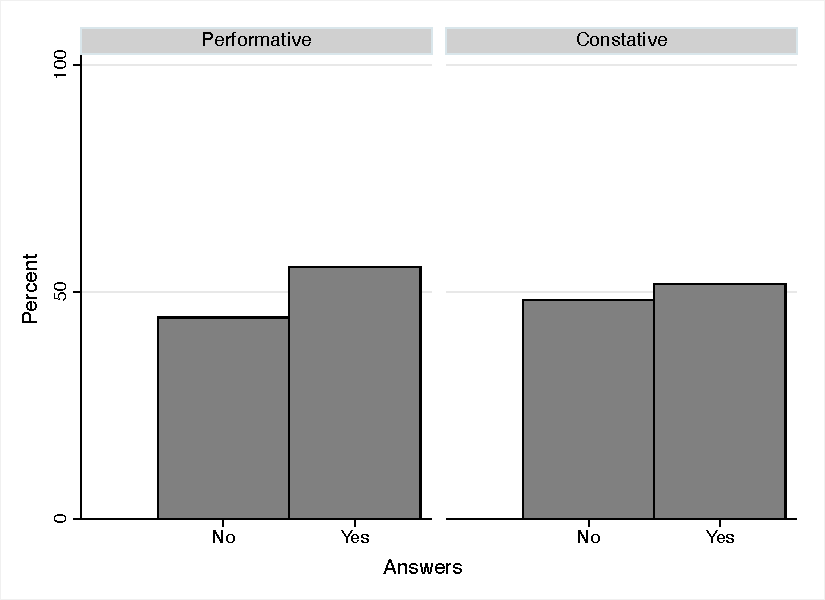
\includegraphics[width=0.1\textwidth]{figures/beha_1.pdf}   & 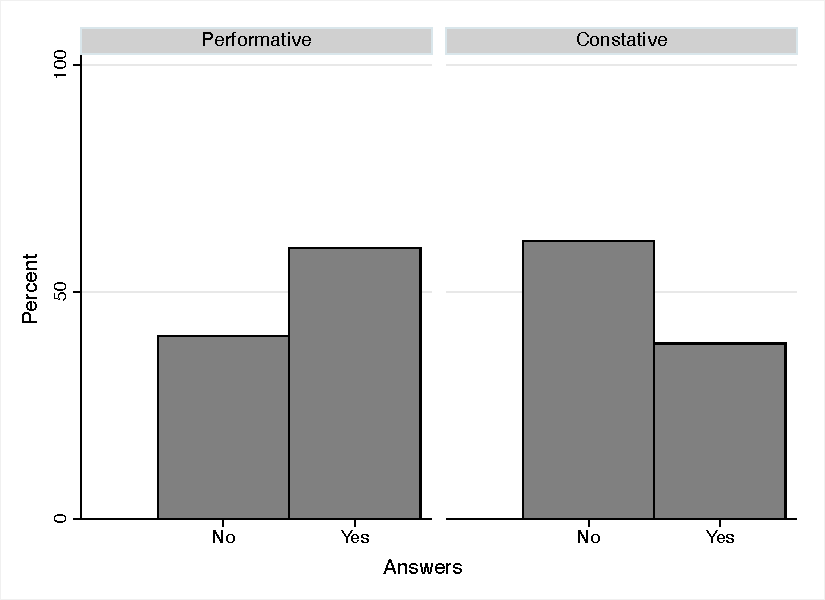
\includegraphics[width=0.1\textwidth]{figures/verd_1.pdf}   & 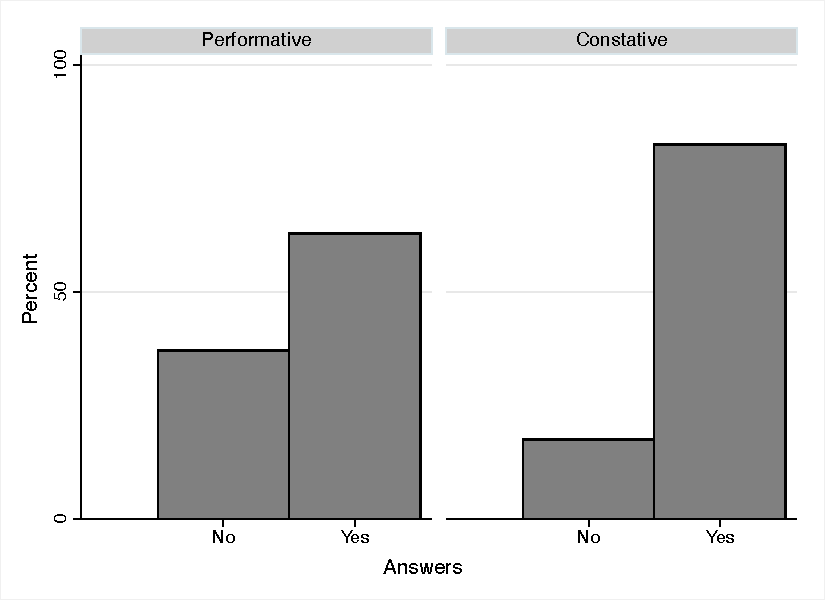
\includegraphics[width=0.1\textwidth]{figures/exer_1.pdf}   & 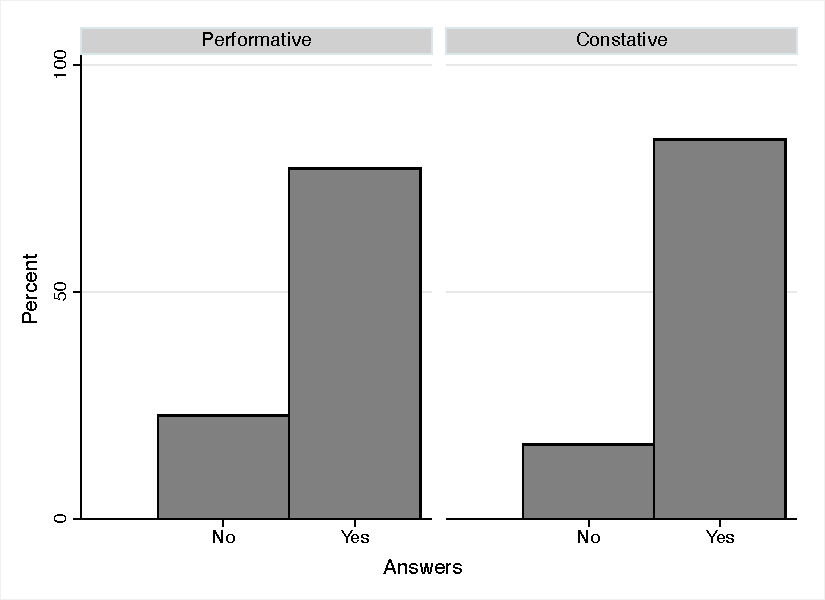
\includegraphics[width=0.1\textwidth]{figures/comm_1.pdf}   & 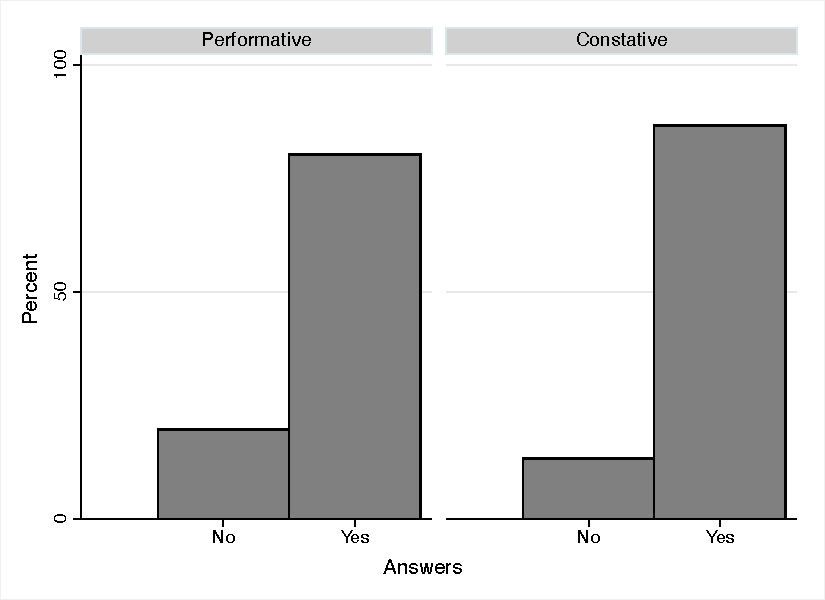
\includegraphics[width=0.1\textwidth]{figures/expo_1.pdf}   \\
Act          & 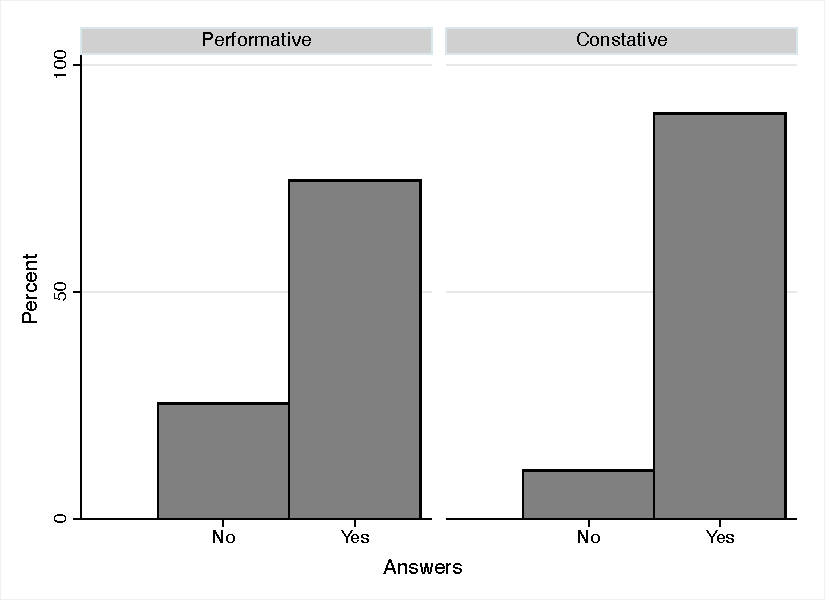
\includegraphics[width=0.1\textwidth]{figures/beha_2.pdf}   & 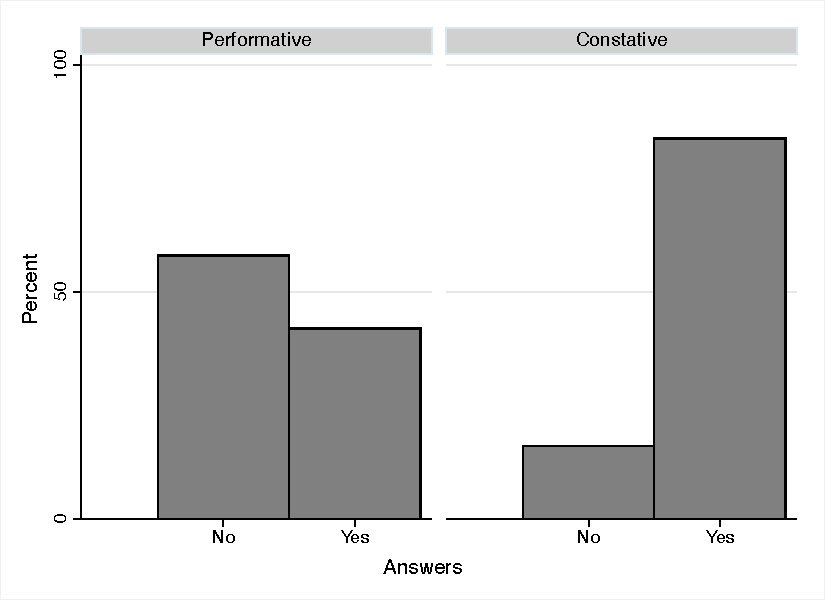
\includegraphics[width=0.1\textwidth]{figures/verd_2.pdf}   & 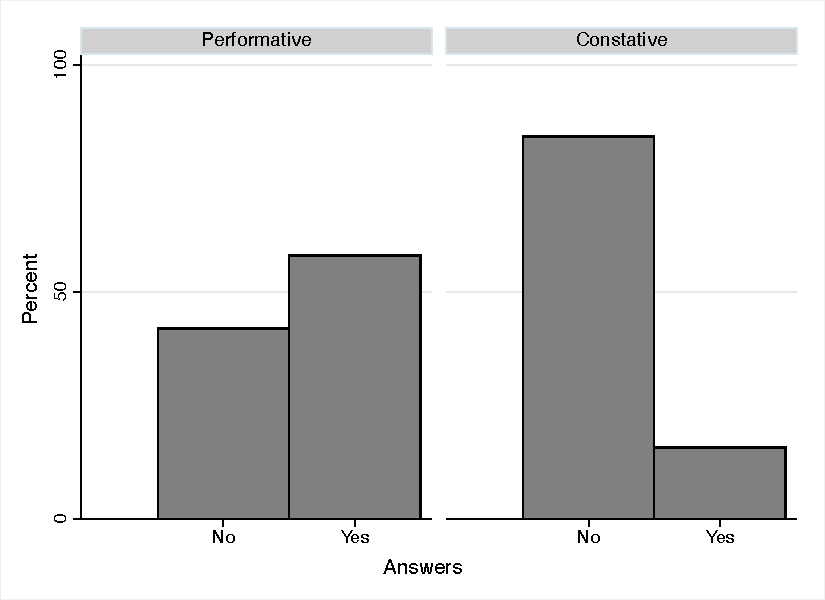
\includegraphics[width=0.1\textwidth]{figures/exer_2.pdf}   & 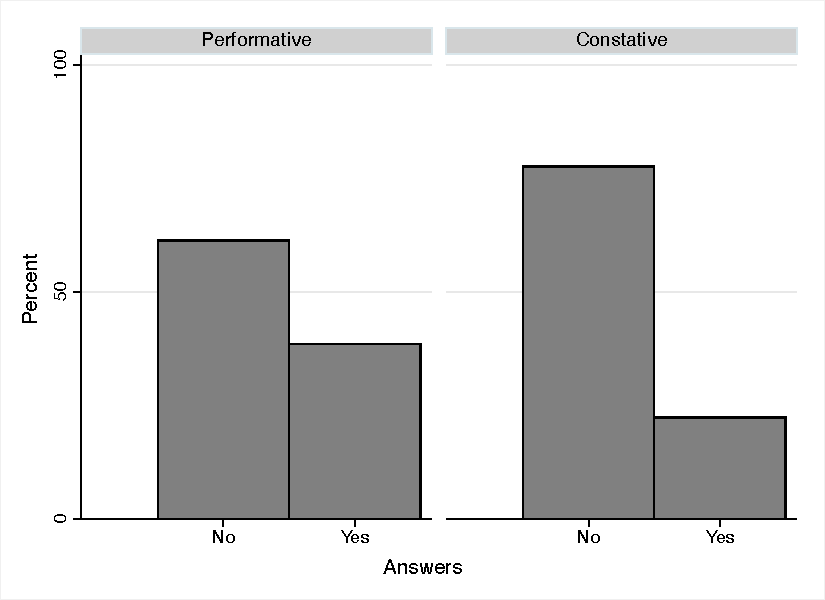
\includegraphics[width=0.1\textwidth]{figures/comm_2.pdf}   & 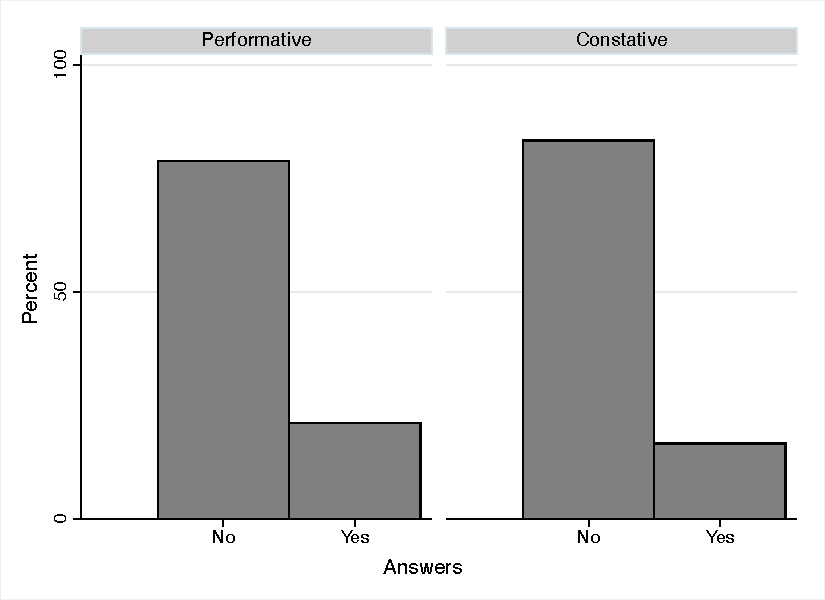
\includegraphics[width=0.1\textwidth]{figures/expo_2.pdf}   \\
Doubt        & 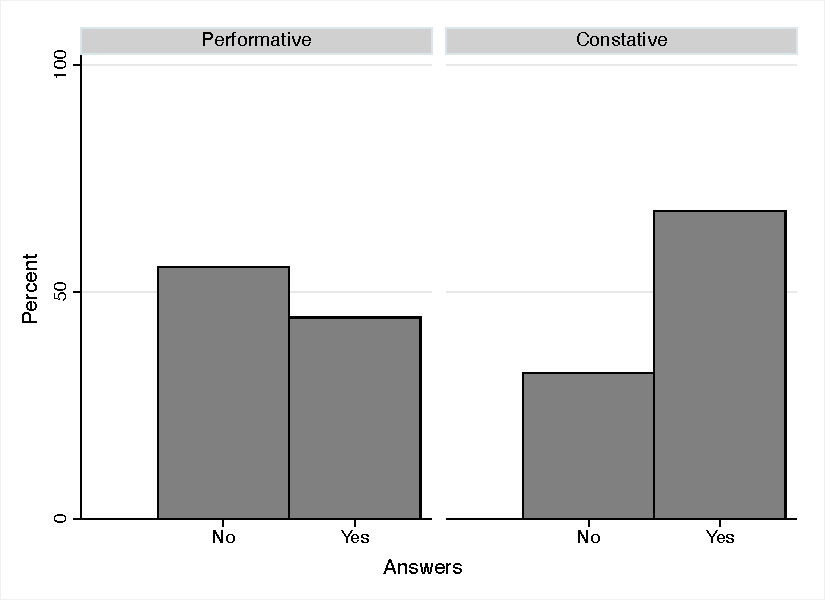
\includegraphics[width=0.1\textwidth]{figures/beha_3.pdf}   & 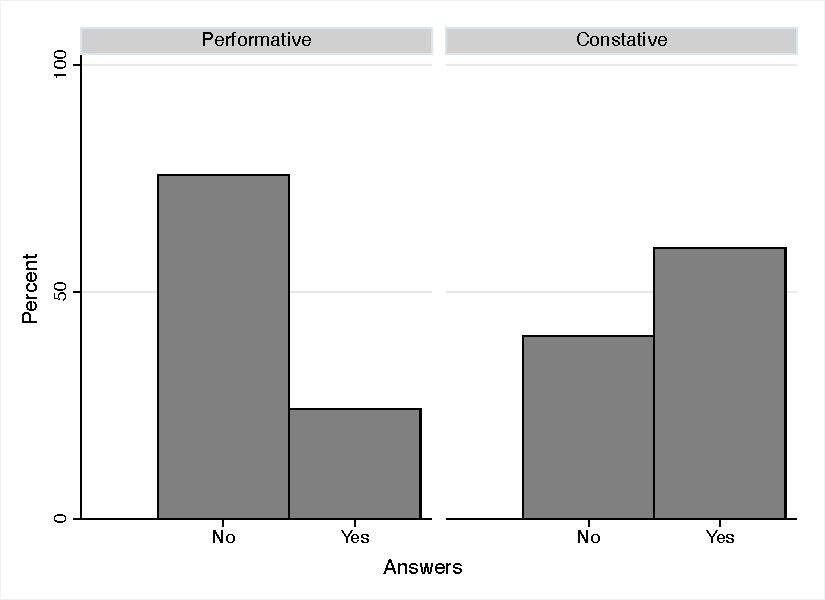
\includegraphics[width=0.1\textwidth]{figures/verd_3.pdf}   & 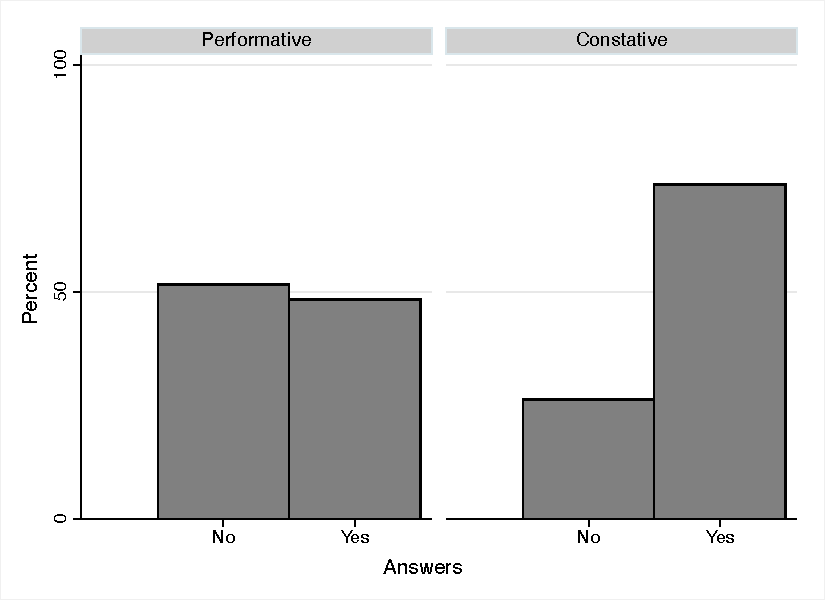
\includegraphics[width=0.1\textwidth]{figures/exer_3.pdf}   & 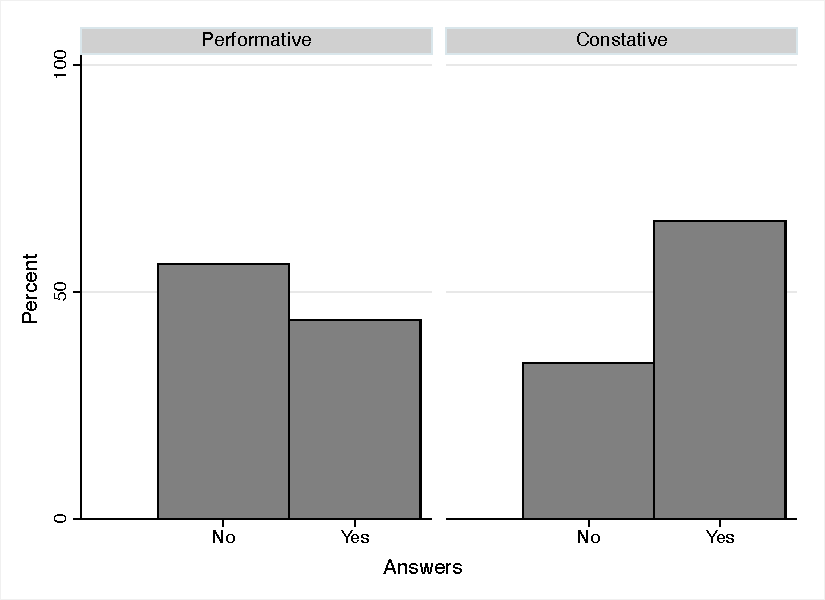
\includegraphics[width=0.1\textwidth]{figures/comm_3.pdf}   & 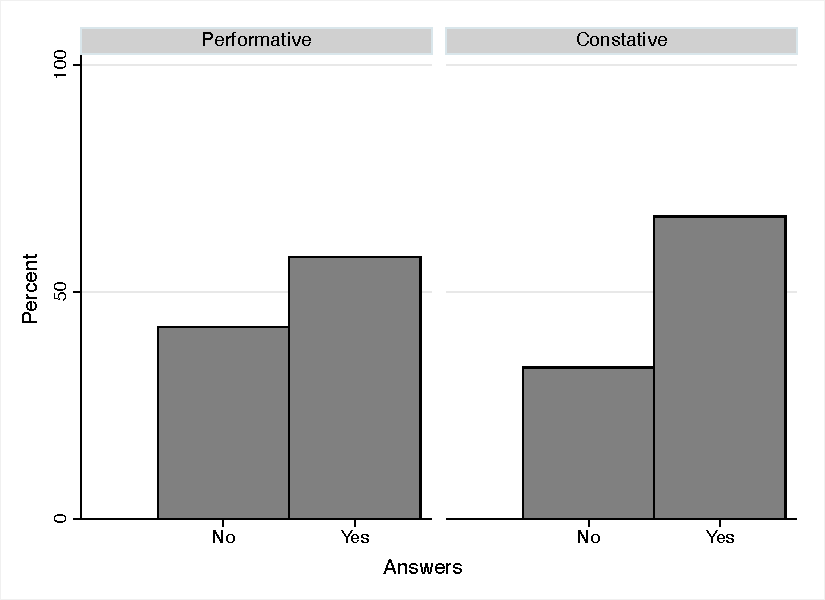
\includegraphics[width=0.1\textwidth]{figures/expo_3.pdf}   \\
Deliberate   & 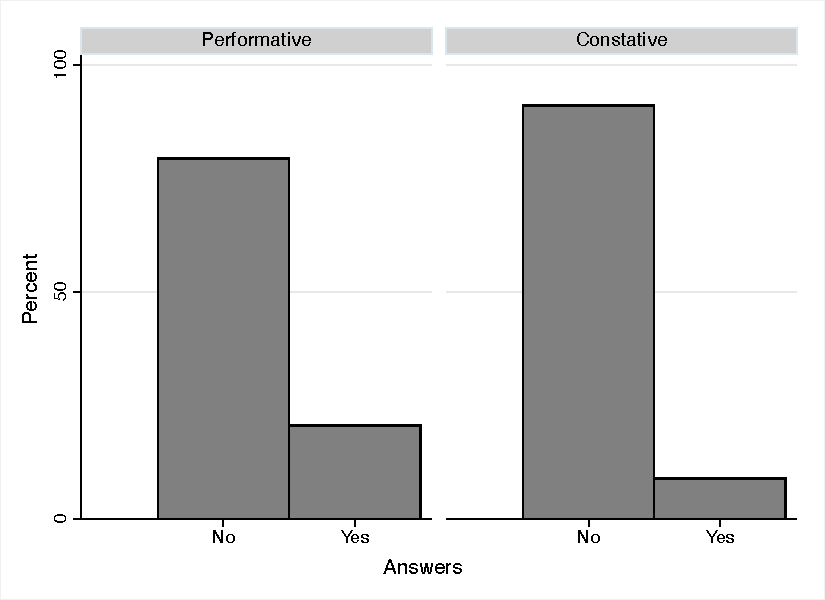
\includegraphics[width=0.1\textwidth]{figures/beha_4.pdf}   & 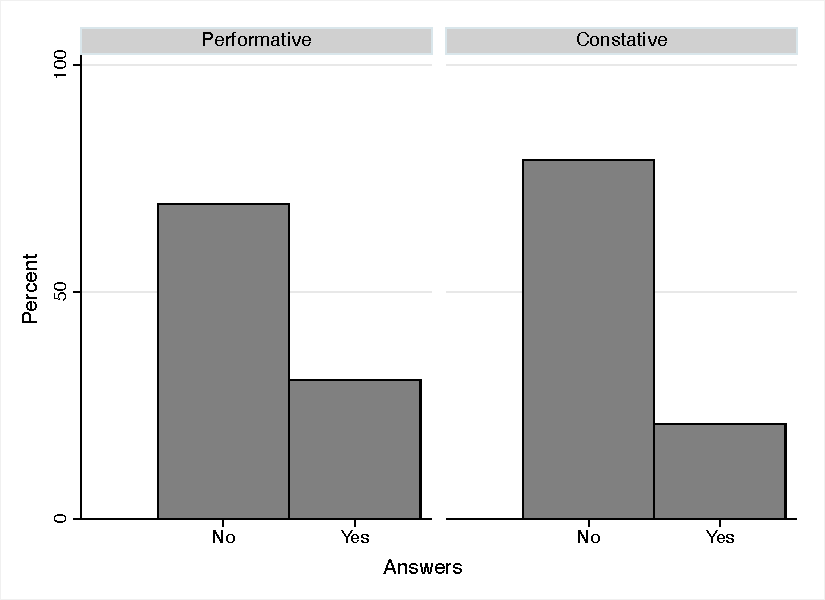
\includegraphics[width=0.1\textwidth]{figures/verd_4.pdf}   & 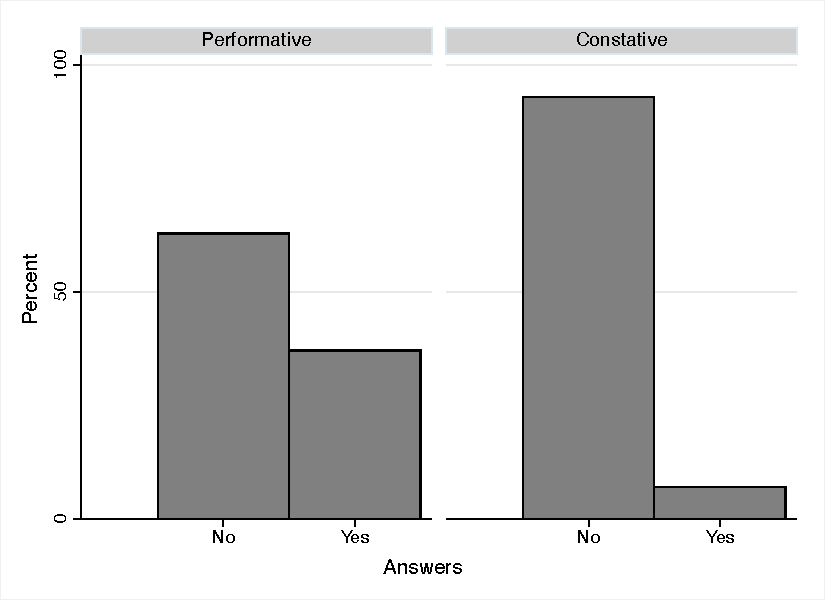
\includegraphics[width=0.1\textwidth]{figures/exer_4.pdf}   & 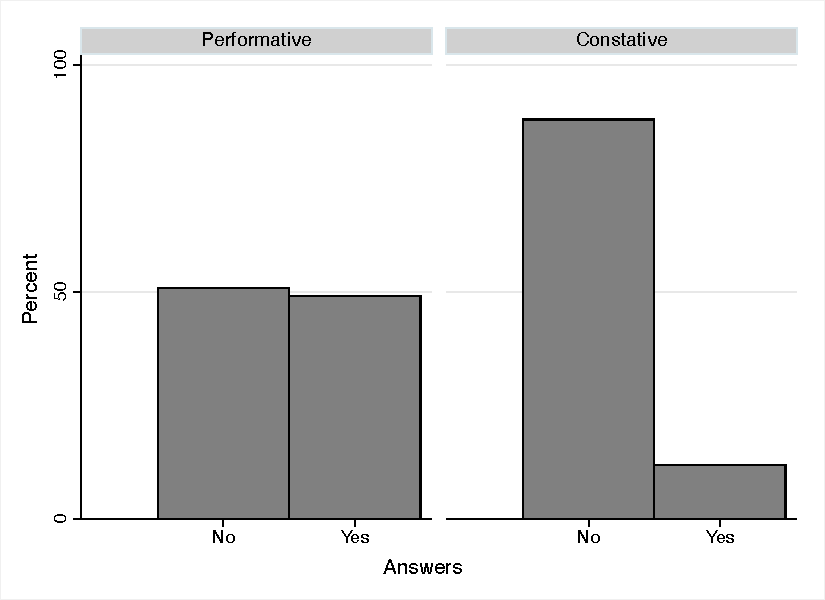
\includegraphics[width=0.1\textwidth]{figures/comm_4.pdf}   & 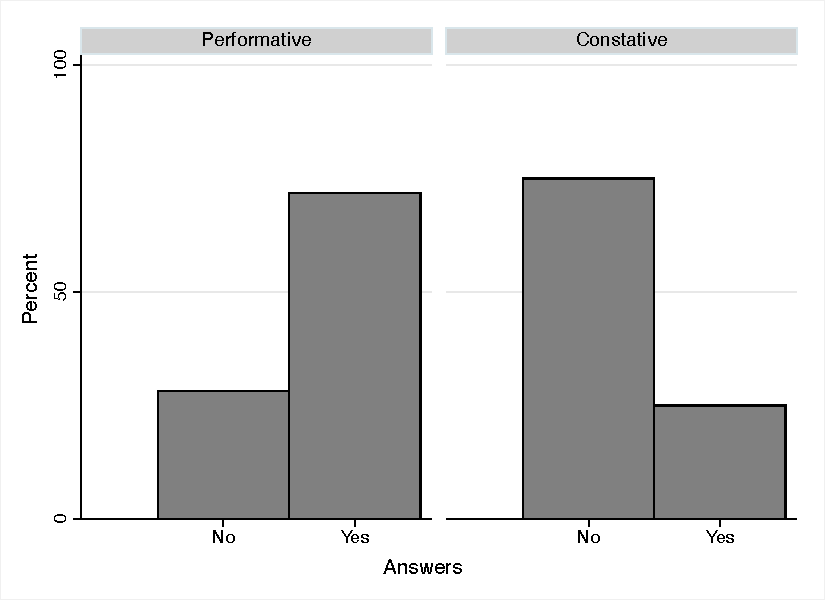
\includegraphics[width=0.1\textwidth]{figures/expo_4.pdf}   \\
Time         & 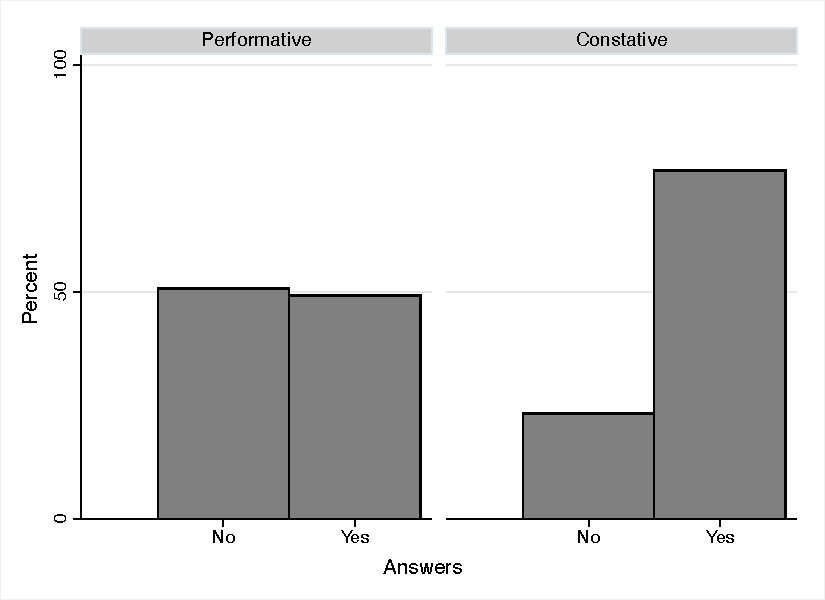
\includegraphics[width=0.1\textwidth]{figures/beha_5.pdf}   & 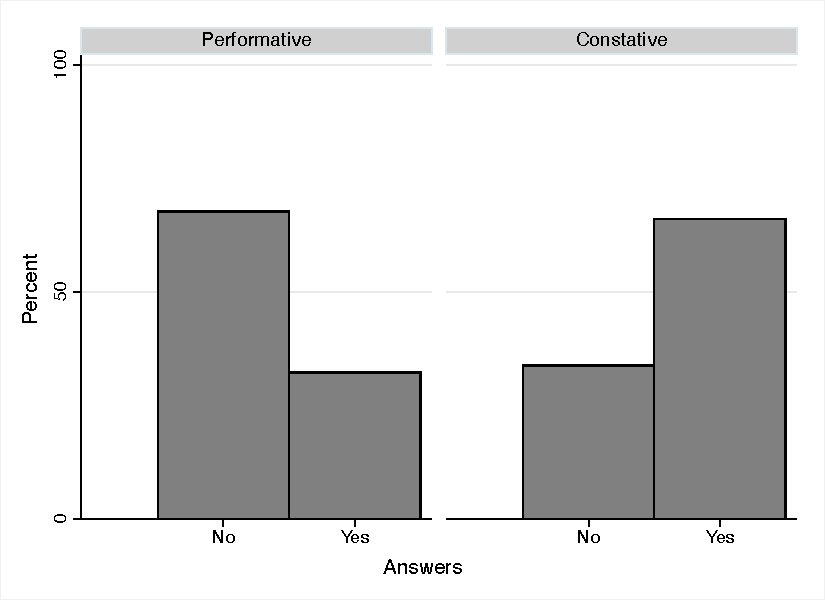
\includegraphics[width=0.1\textwidth]{figures/verd_5.pdf}   & 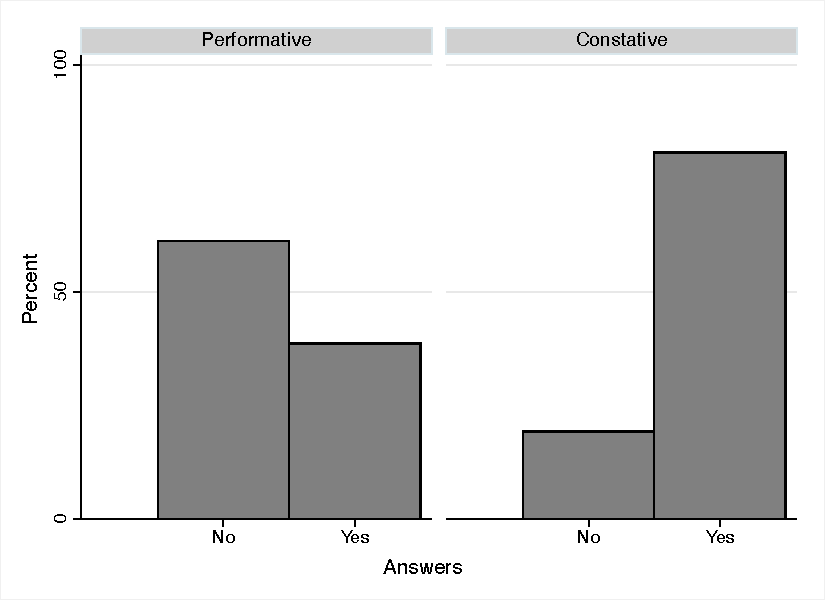
\includegraphics[width=0.1\textwidth]{figures/exer_5.pdf}   & 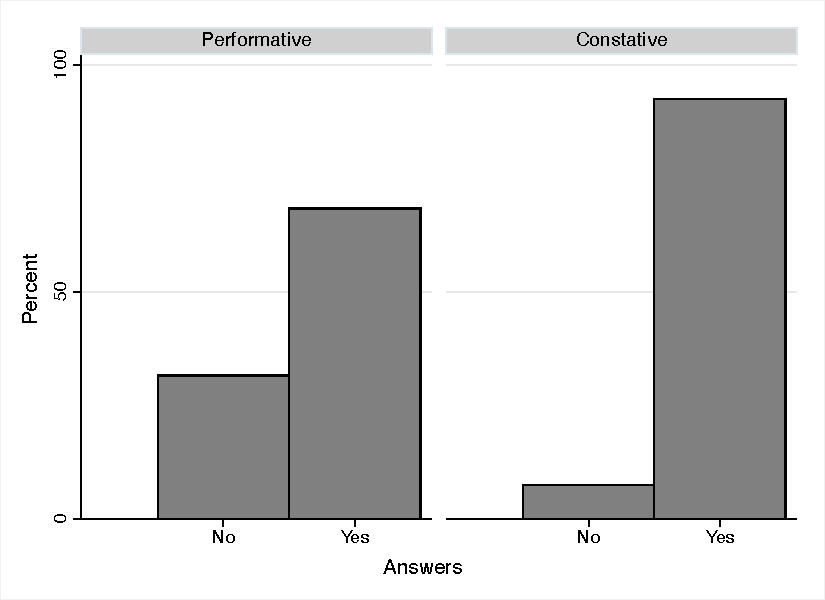
\includegraphics[width=0.1\textwidth]{figures/comm_5.pdf}   & 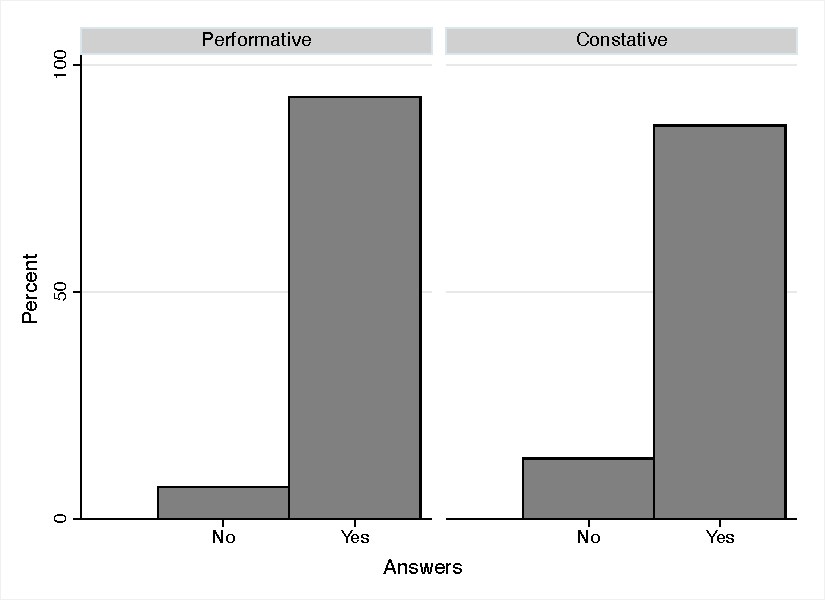
\includegraphics[width=0.1\textwidth]{figures/expo_5.pdf}   \\
\hline
\end{tabular}}
\captionof{figure}{Bar charts of answers}\label{fig:bars}
\end{table}
\end{landscape}


%%%%%%%%%%%%%%%%%%%%
% DISCUSSION AIM 1 %
%%%%%%%%%%%%%%%%%%%%
\subsection{Discussion of Aim 1}
At first, we need to specify under which conditions the responses to a certain criterion and a certain class of performatives should count as being in accordance with Austin's classification (positive case) and under which conditions they do not (negative case). As two first necessary conditions for a positive case, we demand at least a significance level of $p<0.05$ and a small effect size of $|V|>0.1$. This means that presenting a constative and a performative makes a significant difference with respect to the response patterns of native speakers. Evaluating Table \ref{tab:tests}, we obtain the following pattern of positive cases (all empty cells represent negative cases) in Table \ref{tab:tentative_positives}.

\begin{table}[ht]
\begin{tabular}{llllll}
\hline
Question   & Behabitive & Verdictive & Exercitive & Commissive & Expositive \\
\hline\hline
Truth      & positive   & positive   & positive   &            &            \\
Act        &            & positive   & positive   & positive   &            \\
Doubt      & positive   & positive   & positive   & positive   &            \\
Deliberate &            &            & positive   & positive   & positive   \\
Time       & positive   & positive   & positive   & positive   &            \\
\hline\\[-1.5ex]
\multicolumn{6}{p{13.5cm}}{\footnotesize\textit{This table shows the cases in which a class of performatives should count as being in accordance with Austin's classification if we demand at least a significance level of $p<0.05$ and a small effect size of $|V|>0.1$.}}
\caption{Tentative classification of positive cases}\label{tab:tentative_positives}
\end{tabular}
\end{table}

\noindent However, the two conditions (statistical significance and effect size) on their own can hardly be considered sufficient for a positive case. Let's reconsider the question we want to answer in Aim 1: Do native speakers' intuitions regarding Austin's criteria to distinguish between constatives and performatives lead to \textit{the same classification as predicted by Austin's theory of constatives and performatives}? Taking into account the italic part of our question, we additionally need to consider the yes-no patterns of subjects' responses. This can be seen more easily in Figure \ref{fig:bars}. It might be the case that a difference between two treatments is significant and has at least a small effect size, but the yes-no-distribution can be different from Austin's classification. Take, for example, the results of Question Act for the verdictive (line 2, row 2). Here, the $\chi^2$ test shows a highly significant result ($p<0.001$) and a medium effect size ($V=0.434$). However, it would be misleading to count the responses as a positive case because the yes-no-distinction is contrary to Austin's prediction: Subjects tend to judge the constative as being the doing of an action, but not the performative. That is, subjects tend to judge the constative as being a performative and vice versa. Hence, this case should be taken as a negative case. In sum, we define positive cases with respect to the following three necessary and jointly sufficient conditions.\\

\begin{addmargin}[11pt]{0pt}
   \textbf{Definition positive/negative case:} The response pattern to a certain question given a certain class of performatives is a \textit{positive case} if and only if the difference is statistically significant and has at least a small effect size and shows a yes-no-distinction in accordance to Austin's classification. Otherwise, it is a \textit{negative case}.\\
\end{addmargin}

\noindent Given this complete definition of positive and negative cases, we obtain the following Table \ref{tab:final_positives}.

\begin{table}[ht]
\begin{tabular}{llllll}
\hline
Question   & Behabitive & Verdictive & Exercitive & Commissive & Expositive \\
\hline\hline
Truth      &            &            &            &            &            \\
Act        &            &            & positive   &            &            \\
Doubt      & positive   & positive   & positive   & positive   &            \\
Deliberate &            &            &            &            & positive   \\
Time       & positive   & positive   & positive   &            &            \\
\hline\\[-1.5ex]
\multicolumn{6}{p{13.5cm}}{\footnotesize\textit{This table shows the cases in which a class of performatives should count as being in accordance with Austin's classification if we demand at least a significance level of $p<0.05$ and a small effect size of $|V|>0.1$.}}
\caption{Final classification of positive cases}\label{tab:final_positives}
\end{tabular}
\end{table}

\noindent Let's have a closer look at some of our findings. Probably the most surprising result is that the two basic criteria expressed by Question Truth and Question Act hardly seem to work. That is, the results tend to show that native speakers' intuitions with respect to Question Truth and Question Act -- at least in our study's set-up -- do not lead to a classification of constatives and performatives according to Austin (less than 50\% positive cases each). Here, the two most basic criteria do not cause subjects to consistently distinguish between two classes of utterances. The same goes for Question Deliberate that only shows one positive case. Astonishingly, the first of the two fundamental criteria expressed by Question Truth shows no positive cases at all. In the discussion of Aim 4, we will present a possible explanation of this finding.

However, the responses to Question Doubt show a positive case for each class of performatives except the expositives. Why does this criterion tend to work so much better? In the discussion of Aim 2, we will suggest a uniform explanation of why Question Doubt, as well as Question Time, work better than the other criteria. Further, the question arises why Question Doubt does not work for expositives. The reason might be that expositives are an in some respects divergent class of performatives. In the discussion of Aim 3, we will go into more detail with respect to this point.

In sum, only one of Austin's criteria (Question Doubt) seems to work in most cases we tested (or in all cases if we exclude the responses to expositives for reasons we discuss in Aim 3). With respect to the two most fundamental criteria represented by Question Truth and Question Act, native speakers' judgements do not lead to the same classification as predicted by Austin's theory of constatives and performatives.


%%%%%%%%%%%%%%%%%%%%
% DISCUSSION AIM 2 %
%%%%%%%%%%%%%%%%%%%%
\subsection{Discussion of Aim 2}
As Table \ref{tab:final_positives} shows, Question Time tends to work for the behabitive, the verdictive, and the excercitive. Leaving aside the expositives for reasons we discuss in Aim 3, Question Time works for most of the cases we investigated. It shows almost as many positive cases as Question Doubt. For the behabitive and for the excercitive it even shows a higher level of significance and a larger effect size than Question Doubt. The same applies to the commissive, which, however, does only show a yes-no-distinction in accordance with Austin for the constative and, thus, is not classified as a positive case.

Why do Question Doubt and Question Time show much more ``successful'' results than the other criteria? A possible explanation for the success of both criteria is that both Question Doubt and Question Time focus on the \textit{event character} of performatives and not on having a truth value (Question Truth) or on being an action (Question Act) that -- as every action -- can be performed deliberately (Question Deliberate). Uttering a performative is an event strongly limited in time: Regarding the event of apologizing for something, or of acquitting someone or of pardoning someone, and so on, it does not make sense to ask, ``Do they really apologize, acquit, pardon, and so on?'' because the respective events happen \textit{in uttering} the performative and the events end with the utterance. In the same way, it does not make sense to ask, ``Do they still apologize, acquit, pardon (and so on)?'' because the events of apologizing, acquitting and pardoning are temporally completed in uttering the performative. This gives reason to assume that contrary to Austin, the basic character of a performative is not being an action without a truth value but being an event strongly limited in time.

At this point, one might argue that there actually is no difference between the action character and the event character of performatives, arguing that every action is an event. However, first, not every action is temporally as much restricted as it is the event of uttering a performative (like, for example, the action of climbing a mountain). This is why our specification of performatives as events \textit{strongly limited in time} makes a difference. Second, it might be the case that every action is an event, but the reverse relation does not hold. Hence, being an action is a narrower classification than being an event. It might be the case that conceptualizing performatives as actions might be too narrow to be adequate and that characterizing performatives as events might come closer to what Austin actually hat in mind. 


%%%%%%%%%%%%%%%%%%%%
% DISCUSSION AIM 3 %
%%%%%%%%%%%%%%%%%%%%
\subsection{Discussion of Aim 3}
As we discussed in Section \ref{sec:aims}, Austin's probably strongest argument (the CEA) against the constative--performative distinction says that every constative has an illocutionary force and, hence, is an implicit performative. For example, uttering the constative ``The earth turns around the sun'' actually means to claim, to state, to describe, and so forth, that the earth turns around the sun. That is, every constative can also be an expositive. Do our findings provide some hints on whether the CEA holds? To answer this question, let's have a look at the yes-not patterns of the expositive we compared to a constative (Figure \ref{fig:bars}, Expositive). Except for line 4 (Deliberate), there are no significant distinctions between the expositive and the constative. The reason is that for each of the lines 1, 2, 3, and 5, the yes-no patterns of the expositive compared to the constative are almost identical. For these lines, it seems to make no difference whether we present subjects an expositive or a constative with the same propositional content as the expositive has. One might argue that this fact supports the CEA because this would exactly confirm what Austin predicted: constatives behave like performatives (expositives). However, the opposite is the case. If we consider the yes-no patterns, we can see that the responses do not show the patterns Austin predicted for performatives, but on the contrary, subjects' responses for both the performative (expositive) and the constative show the patterns of constatives. That is, our findings are \textit{not} in accordance with the CEA (constatives are expositives), but they support the opposite direction (expositives are constatives).\footnote{Please note that by challenging Austin's CEA and, by doing so, implicitly supporting the constative--performative distinction, we do not intend to challenge his speech act theory. Rather, our findings can be understood as a reason to keep the constative--performative distinction as a pre-theoretical classification in addition to the speech act theory.} Subjects tend to consider the utterance ``I claim that Leonardo DiCaprio is the most attractive man'' as an utterance with a truth value, not as being an action, as something that can be doubted, and not as a single event in time.\footnote{However, deviating from the patterns of lines 1, 2, 3, and 5, Question Deliberate leads to a pattern as predicted by Austin. This point needs further investigation.} Given this interpretation, it becomes clear why the most successful criteria to distinguish constatives and performatives, i.\,e., Question Doubt, as discussed in Aim 1, and Question Time, as discussed in Aim 2, do not work for the constative--performative distinction of expositives. The reason is that subjects do not consider expositives as performatives but as constatives.


%%%%%%%%%%%%%%%%%%%%
% DISCUSSION AIM 4 %
%%%%%%%%%%%%%%%%%%%%
\subsection{Discussion of Aim 4}
As we saw in the Section 2.4, there is a major controversy regarding whether performatives have a truth value as argued by Lemmon (1962), Quine (1981), Heal (1974), Bach (1975), Graham (1977), and Searle (1989), among others, or not, as Austin says. Our findings tend to support the position against Austin. Figure \ref{fig:bars} (line 1) shows that for each performative, subjects tend to agree that the utterance can be true or false, i.\,e., that it has a truth value. Further, for the performatives presented as exercitives, commisives, and expositives, we find significant differences from an equal distribution of answers using one-sample tests of proportion.\footnote{Behabitive: $Z=0.882$, $p=0.378$; Verdictive: $Z=1.524$, $p=0.128$; Exercitive: $Z=2.032$, $p=0.042$; Commisive: $Z=4.106$, $p<0.001$; Expositive: $Z=5.103$, $p<0.001$.}

Additionally, the behabitive, the commissive, and the expositive even do not show a significant difference between the respective performatives and constatives. That is, for these cases, presenting a performative or a constative makes no difference for subjects' responses regarding the question of whether the utterances have truth values. In row 2 of Figure \ref{fig:bars}, a majority even rated the constative not to have a truth value as opposed to the performative. In sum, as far as we can see from our results, subjects tend to disagree with Austin's intuition about performatives concerning the question of whether performatives have truth values. This might be the reason why Question Truth does not work as a criterion to distinguish constatives and performatives, as discussed in Aim 1.

\section{Some Possible Objections}\label{sec:objections}
To our knowledge, this study is the first experimental investigation of Austin's distinction between constative and performative utterances in the experimental philosophy of language. Thus, lacking a generally accepted standard of the experimental design for investigating the distinction between constatives and performative, in this section, we will anticipate and discuss some possible objections. \\

\noindent\textbf{The vignettes and items we used are challengable:} A possible objection is that the items we used as constative and performative utterances in the vignettes are too difficult to interpret. Hence, we should have only used very clear cases of constatives and performatives like, for example, ``Hans and Petra had an accident'' or ``I congratulate you''. We respond to this possible objection that, first, most of the items we used are simple and clear cases of constatives and performatives. Take, for example, the behabitive ``I apologize for the accident'' and the corresponding constative ``I regret the accident''. Second, constatives and performatives are always utterances, i.\,e., they should be presented as part of a conversation and not isolated from context. Otherwise, relevant context information is missing – for example, it is important to know that it is a judge saying ``I hereby acquit you'' and not someone else. However, to ensure that the results are not confounded by different contexts presented to the subjects, we chose pairs of one constative and one performative that could be uttered in one and the same conversational context (at least for all but one of the vignettes). On the contrary, contrasting very clear cases like ``Hans and Petra had an accident'' and ``I congratulate you'' would require different contexts. However, different contexts would confound our results because the differences in the responses that we would possibly measure could be due to the different contexts or due to the different utterances or due to both. Therefore, we created vignettes that do not change the context. However, the price to pay for keeping the context constant is that we could not use the easiest possible utterances (as you can see, for example, for our commissives).\\

\noindent\textbf{The subjects should have been trained/instructed how to understand the test questions:} A second possible objection is that the responses the subjects gave to our test questions do not reflect what we actually wanted to find out because subjects do not understand the question in the way we intended them to be understood. For example, in the case of ``I apologize for the accident'', the questions ``Can the utterance be true or false?'' (Question Truth) or ``Does it make sense to ask whether Hans really apologized for the accident?'' (Question Doubt) could \textit{also} be understood as whether the speaker was making a sincere apology or not. Hence, one could say, before doing the actual survey, subjects should be trained or instructed how to understand the test questions. That is, subjects should be instructed that we are interested in a correspondence reading of truth regarding Question Truth and that we are interested whether the doing of an action by uttering a performative could really be doubted. When we developed the experimental design, we extensively discussed this point. However, we discarded such a proceeding although it would probably have led to clearer results. Why that? Our intention is to test the intuitions of native speakers regarding Austin's tests to distinguish constatives and performatives and to find out whether there is evidence in favor of the constative--performative distinction, i.\,e., whether \textit{constative} and \textit{performative} are pragmatic categories in language. Making the test subjects aware of the distinction between constatives and performatives by instructing them how to understand and how to use the test questions would be like implementing the constative--performative distinction before testing whether it exists in the linguistic representation of the test subjects. Our study is settled within the philosophy of normal language. That is, we use vignettes and questions in normal language in order to explore normale language. Subsequently, if we want to find out, whether, for example, the question ``Does it make sense to ask whether Hans really apologized for the accident?'' is a useful tool to identify performatives, we should not teach subjects how they should understand the question. In doing so we would leave the philosophy of normal language (at least in a narrow sense) and we would teach them the difference between constatives and performatives indirectly. However, we acknowledge that there also can be good reasons to use a different experimental setup.\\ 

\noindent\textbf{Our study does not refer to Austin's speech act theory and, hence, is philosophically irrelevant because Austin replaced the constative--performative distinction with the speech act theory:} A third possible objection is that our study is philosophically irrelevant because it is not concerned with Austin's speech act theory and because it would be mistaken to call the constative--performative distinction a theory at all. It is true that we are not concerned with Austin's speech act theory. However, we do not think that this is a shortcoming. The constative--performative distinction is of significant interest for pragmatics and brought up important debates (as we exemplarily pointed out in Section 2.4). Hence, the constative--performative distinction can be understood as a field of research on its own that can be investigated independently of the speech act theory. Further, in his twelves lecture, Austin (1962, p. 147) stresses that the constative--performative distinction stands ``as the \textit{special} theory to the \textit{general} theory'' of speech acts. Thus, we are in accordance with Austin to call it a \textit{theory} and to explore it empirically. However, by exploring the \textit{special theory} we do not want to argue against the speech act theory or deny that the speech act theory is the more elaborated theory. We just focus on the starting point of Austin's line of thought. With Aim 3 we investigate a certain aspect of this relation. However, with respect to the third possible objection, we agree that the speech act theory is of major philosophical relevance and definitely deserves empirical research (in addition to, but not instead of the constative--performative distinction).\\ 


%%%%%%%%%%%%%%
% CONCLUSION %
%%%%%%%%%%%%%%
\section{Conclusion}\label{sec:conclusion}
In the light of John L. Austin's theoretical distinction, we set out to empirically investigating speakers' intuitions about constative and performative utterances. Specifically, we investigated whether native speakers' intuitions are in accordance with Austin's classification of constative and performative utterances (Aim 1), introduced a new criterion for distinguishing between constatives and performatives and investigated whether native speakers classify utterances by means of this criterion (Aim 2), discussed Austin's presumably strongest argument to reject the constative--performative distinction based on the evidence we obtained for Aim 1 and Aim 2 (Aim 3) and evaluated the evidence we obtained in Aim 1 with respect to the question whether performatives have truth values (Aim 4).

With respect to Aim 1 and Aim 2, we found that native speakers' intuitions concerning the constative--performative distinction tend not to conform to Austin's classification except the criterion of Question Doubt. The reason might be that Question Doubt as well as Question Time focus on the event character of performatives. Our findings support the hypothesis that contrary to Austin's assumption that the action character is the essential property of performatives, it might be more adequate to assume that the event character is the fundamental property of performatives. Concerning Aim 3, we found that native speakers do not tend to agree that constatives actually are implicit performatives (expositives), but that expositives tend to be intuitively understood as being constatives. Last but not least, the results of Aim 4 support the philosophers arguing against Austin that performatives have truth values and, hence, are statements.


%%%%%%%%%%%%%%%%%%%
% ACKNOWLEDGMENTS %
%%%%%%%%%%%%%%%%%%%
\section*{Acknowledgments}\label{sec:acknowledgments}
We are indebted to the \textit{Universitätsgesellschaft Oldenburg e.V.} (UGO) for funding this study and to two anonymous reviewers for their valuable comments.


%%%%%%%%%%%%%%
% REFERENCES %
%%%%%%%%%%%%%%
\clearpage
\section*{References}
\begin{itemize}[label=,leftmargin=\parindent,itemindent=-\parindent]
   \item Austin, John L. (1962): \textit{How to do Things with Words}. Oxford: Clarendon.
   \item Bach, Kent (1965): ``Performatives are Statements too.'' \textit{Philosophical Studies} 28(4): 229--236.
   \item Benveniste, Émile (1974): \textit{Probleme der allgemeinen Sprachwissenschaft}. Munich: List.
   \item Black, Max (1963): ``Austin on Performatives.'' \textit{Philosophy} 38(145): 217--226.
   \item Chisholm, Roderick M. (1969): ``Austin's Philosophical Papers.'' In \textit{Symposium on J. L. Austin}, ed. K. T. Fann, 101--126. London: Routledge \& Kegan Paul.
   \item Cohen, Jacob (1988): \textit{Statistical Power Analysis for the Behavioral Sciences}. 2. ed. Hillsdale: L. Erlbaum Associates.
   \item Forguson, Lynd W. (1966): ``In Pursuit of Performatives.'' \textit{Philosophy} 41(158): 341--347.
   \item Graham, Keith (1977): \textit{J. L. Austin. A Critique of Ordinary Language Philosophy}. Hassocks: Harvester.
   \item Hansen, Nat, and Emmanuel Chemla (2015). ``Linguistic Experiments and Ordinary Language Philosophy.'' \textit{Ratio} 28(4): 422--445.
   \item Heal, Jane (1974): ``Explicit Performative Utterances and Statements.'' \textit{The Philosophical Quarterly} 24(95): 106--121.
   \item Hornsby, Jennifer (2006): ``Speech Acts and Performatives.'' In \textit{The Oxford Handbook of Philosophy of Language}, eds. E. Lepore and B. C. Smith, 893--909. Oxford: Oxford University Press.
   \item Katz, Jerrold J. (1977): \textit{Propositional Structure and Illocutionary Force}. Sussex: Harvester.
   \item Lemmon, Edward J. (1962): ``On Sentences Verifiable by their Use.'' \textit{Analysis} 22(4): 86--89.
   \item LimeSurvey (2020): \textit{LimeSurvey. An Open Source Survey Tool}. Hamburg: LimeSurvey Project.
   \item Quine, Willard Van Orman (1981): \textit{Theories and Things}. Cambridge and London: The Belknap Press of Harvard University Press.
   \item Searle, John R. 1975. ``A Taxonomy of Illocutionary Acts.'' In Minnesota Studies in the Philosophy of Science 9: Language, Mind and Knowledge, ed. K. Gunderson, 344--368. Minneapolis: University of Minnesota Press.
   \item Searle, John R. (1989): ``How Performatives Work.'' \textit{Linguistics and Philosophy} 12: 535--558.
   \item Sesonske, Alexander (1965): ``Performatives.'' \textit{The Journal of Philosophy} 62: 459--468.
   \item Siebel, Mark (2002): ``What is a Illocutionary Point?'' In \textit{Speech Acts, Mind, and Social Reality. Discussions with John R. Searle}, eds. G. Grewendorf and G. Meggle, 124--140. Dordrecht: Kluwer.
   \item Soames, Scott (2003): \textit{Philosophical Analysis in the Twentieth Century. Vol. 2: The Age of Meaning}. Princeton: Princeton University Press.
   \item Tsohatzidis, Savas L. (2018): ``Performativity and the `True/False Fetish'.'' In \textit{Interpreting J. L. Austin}, ed. S. L. Tsohatzidis, 96--118. Cambridge: Cambridge University Press.
   \item Warnock, Geoffrey J. (1973): ``Some Types of Performative Utterance.'' In \textit{Essays on J. L. Austin}, ed. I. Berlin, 69--89. Oxford: Clarendon.
   \item Zahorec, Michael, Robert Bishop, Nat Hansen, John Schwenkler, and Justin Sytsma (forthcoming): ``Linguistic Corpora and Ordinary Language. On the Dispute between Ryle and Austin about the Use of `Voluntary', `Involuntary', `Voluntarily', and `Involuntarily'. In: David Bordonaba: \textit{Experimental Philosophy of Language. Perspectives, Methods and Prospects}. Dordrecht: Springer.
\end{itemize}


%%%%%%%%%%%%
% APPENDIX %
%%%%%%%%%%%%
\clearpage
\appendix
\section{Instructions and Questions of the Study}\label{sec:app_instructions}


%%%%%%%%%%%%%%%%%%%
% WELCOME MESSAGE %
%%%%%%%%%%%%%%%%%%%
\subsection{Welcome Message}\label{sec:app_welcome}
Welcome to our study!

If you work in a concentrated manner, you will probably not need more than 5 to 10 minutes for this study. It is important that you read the instructions and tasks carefully. Also, please complete the study without closing your browser in between.

We will evaluate your answers and the answers of all other participants in this study. All data will be stored in anonymous form, so that no information can be assigned to a single person. The results of the study will be published.

Thank you for your participation!


%%%%%%%%%%%%%%%%
% INSTRUCTIONS %
%%%%%%%%%%%%%%%%
\subsection{Instructions}\label{sec:app_instructions}
In this study, you will be presented with a verbal utterance that someone says in a certain situation. You will then be asked to answer a total of five yes-or-no questions about this utterance. Please answer the questions according to your own personal assessment. There are no right or wrong answers.


%%%%%%%%%%%%%
% QUESTIONS %
%%%%%%%%%%%%%
\subsection{Questions}\label{sec:app_questions}
\noindent\textit{Note: Questions were displayed in randomized order.}

\vspace{1ex}
\noindent\textbf{Question 1:} Can the utterance be true or false?

\vspace{1ex}
\noindent\textbf{Question 2:} Does Hans [the judge/the president/Petra] perform an action with the utterance (in addition to the action of speaking)?

\vspace{1ex}
\noindent\textbf{Question 3:} Does it make sense to ask whether Hans really apologized for the accident [Hans really regretted the accident/the judge really acquitted the defendant/the judge really thought the defendant was innocent/the president really pardoned the detainee/the president really thought the detainee should be pardoned/Petra really promised to go to the movies with Hans/Petra really intended to go to the movies with Hans/Petra really claimed that Leonardo DiCaprio is the most attractive man/Petra really thinks that Leonardo DiCaprio is the most attractive man] (i.\,e., can one doubt that he apologized for the accident [he regretted the accident/the judge acquitted the defendant/the judge thought the defendant was innocent/the president pardoned the detainee/the president thought the detainee should be pardoned/she promised to go to the movies with him/she intended to go to the movies with him/she really claimed that Leonardo DiCaprio is the most attractive man/she really thinks that Leonardo DiCaprio is the most attractive man])?

\vspace{1ex}
\noindent\textbf{Question 4:} A week later, Hans [the judge/the president/Petra] tells a friend about his conversation with Petra [the trial/the meeting with the prisoner/her conversation with Hans].

While doing so, can he [she] insert the word ``deliberately'' into his [her] report without making it nonsensical?

The report would then be: ``I deliberately apologized for the accident [I deliberately regretted the accident/I deliberately acquitted the defendant/I deliberately believed the defendant to be innocent/I deliberately pardoned the detainee/I deliberately thought the detainee should be pardoned/I deliberately promised to take him to the movies/I deliberately intended to go to the movies with him/I deliberately claimed that Leonardo DiCaprio is the most attractive man/I deliberately thought Leonardo DiCaprio is the most attractive man].''

\vspace{1ex}
\noindent\textbf{Question 5:} Does it make sense to ask a week later if Hans is still apologizing for the accident [Hans is still regretting the accident/the judge is still acquitting the defendant/the judge is still thinking the defendant is innocent/the president is still pardoning the detainee/the president is still thinking the detainee should be pardoned/Petra is still promising to go to the movies with Hans/Petra is still intending to go to the movies with Hans/Petra is still claiming that Leonardo DiCaprio is the most attractive man/ Petra is still thinking that Leonardo DiCaprio is the most attractive man]?


%%%%%%%%%%%%%%%%%%%%
% CONTROL QUESTION %
%%%%%%%%%%%%%%%%%%%%
\subsection{Control Question}\label{sec:app_control}
Which of the following questions about Hans' [the judge's/the president's/Petra's] utterance were you not asked in this survey?

\begin{itemize}
\item[$\square$]Does Hans [the judge/the president/Petra] perform an action with the utterance (in addition to the action of speaking)?

\item[$\square$]Can the utterance be true or false?

\item[$\square$]Does it make sense to ask whether Hans really apologized for the accident [Hans really regretted the accident/the judge really acquitted the defendant/the judge really thought the defendant was innocent/the president really pardoned the detainee/the president really thought the detainee should be pardoned/Petra really promised to go to the movies with Hans/Petra really intended to go to the movies with Hans/Petra really claimed that Leonardo DiCaprio is the most attractive man/Petra really thinks that Leonardo DiCaprio is the most attractive man] (i.\,e., can one doubt that he apologized for the accident [he regretted the accident/the judge acquitted the defendant/the judge thought the defendant was innocent/the president pardoned the detainee/the president thought the detainee should be pardoned/she promised to go to the movies with him/she intended to go to the movies with him/Petra really claimed that Leonardo DiCaprio is the most attractive man/Petra really thinks that Leonardo DiCaprio is the most attractive man])?

\item[$\square$]Does it make sense to ask a week later if Hans is still apologizing for the accident[Hans is still regretting the accident/the judge is still acquitting the defendant/the judge is still thinking the defendant is innocent/the president is still pardoning the detainee/the president is still thinking the detainee should be pardoned/Petra is still promising to go to the movies with Hans/Petra is still intending to go to the movies with Hans/Petra is still claiming that Leonardo DiCaprio is the most attractive man/Petra is still thinking that Leonardo DiCaprio is the most attractive man]?

\item[$\square$]Does it make sense to ask whether Hans' [the judge's/the president's/Petra's] utterance is grammatically correct?
\end{itemize}

\end{document}
